\documentclass[../book.tex]{subfiles}

\chapter{Diagramming machines}
\label{ch:diagram}

\begin{quote}
Machine learning is not magic; it cannot get something from nothing.
What it does is get more from less. Programming, like all engineering,
is a lot of work: we have to build everything from scratch. Learning is
more like farming, which lets nature do most of the work. Farmers
combine seeds with nutrients to grow crops. Learners combine knowledge
with data to grow programs. \autocite[81]{Domingos_2012}
\index{Domingos, Pedro}
\end{quote}

\begin{quote}
The tools or material machines have to be chosen first of all by a
diagram \autocite[39]{Deleuze_1988} \index{Deleuze, Gilles}
\index{diagram}
\end{quote}

The `learning' in machine learning embodies a change in programming
practice or indeed the programmability of machines. Our sense of the
potentials of machine learning can be understood, according to Pedro
Domingos, in terms of a contrast between programming as `a lot of
{[}building{]} work' and the `farming' done by machine learners to `grow
programs.' In characterising machine learning, the tensions between the
programming `we' (programmers, computer scientists?) do and the
programming that learners do (`growing') are worth pursuing.
\index{programming!human vs. machine} While Domingos suggests that
machine learners `get more from less,' I will propose that an immense
constellation of documents, software, publications, blog pages, books,
spreadsheets, databases, data centre architectures, whiteboard and
blackboard drawings, and an inordinate amount of talk and visual media
orbit around machine learning. \index{programmability!problem of} There
has been lively growth in machine learning, but this liveliness and the
sometimes life-like growth of machine learners are a regional expression
of a distributed formation. `Wherever there is a region of nature,' the
philosopher Alfred North Whitehead writes `which is itself the primary
field of the expressions issuing from each of its parts, that region is
alive' \autocite[31]{Whitehead_1956}.
\index{Whitehead, Alfred North!life}

In this chapter I attend to the problem of identifying and describing
the distributed practices that give rise to a sense of machine learners
framed as growth, or liveliness. I will argue these practices can only
be traced partially through code written in generic or specialized
programming languages such as \texttt{Python} and \texttt{R}, in
libraries of machine learning code such as \texttt{R}'s \texttt{caret}
\index{R!packages!\texttt{caret}} or \texttt{Python}'s
\texttt{scikit-learn} \index{Python!packages!\texttt{scikit-learn}} or
\texttt{TensorFlow} \index{Google!TensorFlow} to do machine learning.
Code obscures and reveals multiple transformations at work in the
operational formation. Science studies scholars such as Anne-Marie Mol
have urged the need to keep practice together with theories of what
exists. Mol writes:

\begin{quote}
If it is not removed from the practices that sustain it, reality is
multiple. This may be read as a description that beautifully fits the
facts. But attending to the multiplicity of reality is also an act. It
is something that may be done -- or left undone \autocite[6]{Mol_2003}
\index{Mol, Anne-Marie}
\end{quote}

Mol advocates thinking reality as multiplicity. Her insistence on the
nexus of practice or doing and the plural existence of things suggests a
way of handling the code that machine learners produce. \index{practice}
Code should be approached multiplicity. In the case of machine learners,
this means following through pedagogical expositions of machine learning
focused on both mathematical derivations and the accumulation of
scientific or technical research publications, ranging from textbooks to
research articles, that vary, explore, experiment and implement machine
learners in code. The effect of liveliness or growth issues from many
parts. In relation to machine learning, reading and writing code
alongside scientific papers, Youtube lectures, machine learning books
and competitions is not only a form of observant participation, but
directly forms part of the diagrammatic multiplicity.

While machine learning utterly depends on code, I will suggest therefore
that no matter how expressive or well-documented it may be, code alone
cannot fully \gls{diagram} how machine learners make programs or how
they combine knowledge with data. Domingos writes that `learning
algorithms \ldots{} are algorithms that make other algorithms. With
machine learning, computers write their own programs, so we don't have
to' \autocite[6]{Domingos_2015a}. Yet the writing performed by machine
learners cannot be read textually or procedurally as other programs
might be read for instance in work known as critical code studies. The
difference between the reading of an Atari computer game console in Nick
Montfort and Ian Bogost's \emph{Racing the Beam}
\autocite{Montfort_2009} and the machine learning of Atari's games
undertaken by DeepMind in London during recent years
\autocites{Mnih_2013}{Mnih_2015} is hard to read from program code.
\index{code!readability of} The learning or making by learning is far
from homogeneous, stable or automatic in practice. Materially, code is
only one element in the diagram of machine learning. It displays, with
greater or lesser degrees of visibility relations between a variety of
forces (infrastructures, scientific knowledges, mathematical
formalisations, etc.). It itself is aligned by and exposes other
institutional, infrastructural, epistemic and economic positions.
\index{code!agency of}

Coding practices and the pedagogical expositions of machine learning
have shifted substantially over the last decade or so due to the growth
in open source programming languages and as a part of the broader and
well-known expansion of digital media cultures. The fact that data
scientists, software developers and other machine learners across
scientific and commercial settings use programming languages such as
\texttt{Python} and \texttt{R}
\index{Python|seealso{programming language}}
\index{R|seealso{programming language!R}} more than specialized
commercial statistical and data software packages such as
\texttt{Matlab}, \texttt{SAS} or \texttt{SPSS} \autocite{Muenchen_2014}
is perhaps symptomatic of shifts in computational culture. Coding
cultures are crucial to the recent growth of machine learning. Although
scientific computing languages such as \texttt{FORTRAN} -- `Formula
Translator' -- have long underpinned scientific research and engineering
applications in various fields
\autocite[34-35]{Campbell-Kelly_2003},\index{programming languages!FORTRAN}
the development in recent decades of data-analytic and statistical
programming languages and coding frameworks has crystallized a
repertoire of standard operations, patterns and functions for reshaping
data and constructing models that classify and predict events and
associations between things, people, processes, etc. This development
continues apace, especially in research and engineering driven by social
media and internet platforms such as Facebook and Google. While Domingos
speaks of `growing' programs, the accumulating sediment of certain
well-established data practices are the soil in which programs take
root. The different elements of coding practice are precisely the
faceted levels of abstraction which we need to access and traverse in
order to know and come to grips empirically with contemporary
compositions of power and knowledge in machine learning.
\index{code!writing of}

\section{\texorpdfstring{`We don't have to write
programs'?}{We don't have to write programs?}}\label{we-dont-have-to-write-programs}

In machine learning, coding changes from what we might call symbolic
logical diagrams to statistical algorithmic diagrams. While many machine
learning techniques have long statistical lineages (running back to the
1900s in the case of Karl Pearson's development of the still-heavily
used Principal Component Analysis \autocite{Pearson_1901}),
\index{Pearson, Karl}\index{machine learner!principal component analysis}
machine learning techniques often embody a certain dissatisfaction with
the classical computer science understanding of programs as manipulation
of symbols, even as they rely on such symbolic operations to function.
Symbolic manipulation, epitomised by deductive logic or predicate
calculus, was very much at the centre of many AI projects during the
1950s and 1960s \autocites{Dreyfus_1972}{Edwards_1996}.
\index{artificial intelligence!symbolic manipulation in} In machine
learning, the privileged symbolic-cognitive forms of logic are subject
to a statistical transformation.

Take for instance once of the most common operations of the Boolean
logical calculus, the \texttt{NOT-AND} or \texttt{NAND} function shown
in table \ref{tab:boolean}. The truth table summarises a logical
function \index{function!logical} that combines three input variables
\texttt{X1}, \texttt{X2}, and \texttt{X3} and produces the output
variable \texttt{Y}. Because in Boolean calculus, variables or
predicates can only take the values \texttt{true} or \texttt{false},
they can be coded in as \texttt{1} and \texttt{0}.

\begin{longtable}[c]{@{}llll@{}}
\caption{The truth table for the Boolean function NOT-AND truth
\label{tab:boolean}}\tabularnewline
\toprule
X1 & X2 & X3 & Y\tabularnewline
\midrule
\endfirsthead
\toprule
X1 & X2 & X3 & Y\tabularnewline
\midrule
\endhead
0 & 0 & 0 & 1\tabularnewline
0 & 0 & 1 & 1\tabularnewline
0 & 1 & 1 & 1\tabularnewline
0 & 1 & 0 & 1\tabularnewline
1 & 0 & 0 & 1\tabularnewline
1 & 0 & 1 & 1\tabularnewline
1 & 1 & 0 & 1\tabularnewline
1 & 1 & 1 & 0\tabularnewline
\bottomrule
\end{longtable}

Now in Foucaultean terms, the truth table and its component propositions
constitutes a statement. This statement has triple relevance for
\gls{archaeology} of machine learning.
\index{statements!truth tables as} The spatial arrangement of the table
is fundamental (and this is the topic of chapter \ref{ch:vector}).
\index{table!see {data!table}} Most datasets come as tables, or end up
as tables at some point in their analysis. Second, the elements or cells
of this table are numbers. The numbers \(1\) and \(0\) are the binary
digits as well as the `truth' values `True' and `False' in classical
logic. These numbers are readable as symbolic logical propositions
governed by the rule \(Y = \neg{X_1 \and X_2 \and X_3}\). The table acts
as a hinge between numbers and symbolic thought or cognition. Third, the
NAND table in particular has an obvious operational relevance in digital
logic, since digital circuits of all kinds -- memory, processing, and
communication -- comprise such logical functions knitted together in the
intricate gated labyrinths of contemporary calculation.\footnote{The
  philosophy Charles Sanders Peirce himself
  \index{Peirce, Charles Sanders!on NAND operation} had first shown that
  combinations of NAND operations could stand in for any logical
  expression whatsoever, thus paving the way for the diagrammatic weave
  of contemporary digital memory and computation in all their
  permutations. Today, NAND-based logic is norm in digital electronics.
  NOR -- NOT OR -- logic is also used in certain applications.}
\index{infrastructure!digital circuit as}

A pre-machine learning programmer, tasked with implementing the logical
NAND function might write:

\begin{lstlisting}[language=Python, caption={XOR function in Python}, label={lst:nand}]
Y = not(X1 & X2 & X3)
\end{lstlisting}

The trivial simplicity of the code stands out. This looks like the kind
of symbol manipulation that that computers can easily be programmed to
do. How, by contrast, could such a truth table be learned by a machine,
even a machine whose \emph{modus operandi} and indeed whose very fabric
is nothing other than a massive mosaic of \texttt{NAND} operations
inscribed in semiconductors? Machine learning of on elementary truth
tables is not a typical operation today, but usefully illustrates
something of the diagrammatic transformations that programming or coding
(and classical AI) has undergone \index{artificial intelligence}.

Machine learners such as decision trees or neural nets typically know
nothing of the logical calculus and its elementary logical operations.
Can they be induced to learn it? A perceptron, an elementary machine
learner dating from the
1950s,\index{machine learner!perceptron!learning logical functions} that
`learns' the binary logical operation NAND (Not-AND) is expressed in
twenty lines of python code on the Wikipedia `Perceptron' page
\autocite{Wikipedia_2013} (see listing \ref{lst:perceptron_code}). It is
a standard machine learner almost always included in machine learning
textbooks and usually taught in introductory machine learning classes.
The code outputs a series of numbers shown in table
\ref{tab:nand_weights}.

\begin{lstlisting}[language=Python, caption={Perceptron learning $XOR$ function}, label={lst:perceptron_code}]

threshold = 0.5
learning_rate = 0.1
weights = [0, 0, 0]
training_set = [((1, 0, 0), 1), ((1, 0, 1), 1), ((1, 1, 0), 1), ((1, 1, 1), 0)]

def dot_product(values):
    return sum(value * weight for value, weight in zip(values, weights))

out = 'weight1, weight2, weight3, error_count, iteration'
print  out
iteration_count = 0
while True:
    error_count = 0
    iteration_count += 1
    for input_vector, desired_output in training_set:
        out = ','.join(map(str,weights)) + ',' + str(error_count)
        out = out + ',' + str(iteration_count)
        result = dot_product(input_vector) > threshold
        error = desired_output - result
        print out
        if error != 0:
            error_count += 1
            for index, value in enumerate(input_vector):
                weights[index] += learning_rate * error * value
    if error_count == 0:
        break
\end{lstlisting}

\begin{table}[!htb]
\centering
\begingroup\tiny
\begin{tabular}{rrrrr}
  \hline
weight1 & weight2 & weight3 & error\_count & iteration \\ 
  \hline
0.00 & 0.00 & 0.00 &   0 &   1 \\ 
  0.10 & 0.00 & 0.00 &   1 &   1 \\ 
  0.20 & 0.00 & 0.10 &   2 &   1 \\ 
  0.30 & 0.10 & 0.10 &   3 &   1 \\ 
  0.30 & 0.10 & 0.10 &   0 &   2 \\ 
  0.40 & 0.10 & 0.10 &   1 &   2 \\ 
  0.50 & 0.10 & 0.20 &   2 &   2 \\ 
  0.50 & 0.10 & 0.20 &   2 &   2 \\ 
  0.40 & 0.00 & 0.10 &   0 &   3 \\ 
  0.50 & 0.00 & 0.10 &   1 &   3 \\ 
  0.50 & 0.00 & 0.10 &   1 &   3 \\ 
  0.60 & 0.10 & 0.10 &   2 &   3 \\ 
  0.50 & 0.00 & 0.00 &   0 &   4 \\ 
  0.60 & 0.00 & 0.00 &   1 &   4 \\ 
  0.60 & 0.00 & 0.00 &   1 &   4 \\ 
   \hline
\end{tabular}
\endgroup
\caption{Iterative change in weights as a perceptron learns the NAND function} 
\label{tab:nand_weights}
\end{table}

What does the code in listing \ref{lst:perceptron_code} show or say
about the transformation in programmability or the writing of programs?
\index{machine learning!as transformation in programming} First of all,
we should note the relative conciseness of the code vignette.
\index{code!brevity in machine learning} Much of the code here is
familiar, generic programming. It defines variables, sets up data
structures (lists of numerical values), checks conditions, loops through
statements or prints results. In citing this code, I am not resorting to
a technical publication or scientific literature as such, or even to a
machine learning software library or package (in \texttt{scikit-learn},
the same model could be written
\texttt{p\ =\ scikit-learn.linearmode.Perceptron(X,Y)}), just to a
Wikipedia page, and the relatively generic and widely used programming
language \texttt{Python}.{[}\^{}1.31{]} Whatever the levels of
abstraction associated with machine learning, the code is hardly ever
hermetically opaque. As statements, everything lies on the surface.
\index{machine learner!perceptron|(}

Second, while the shaping of data, the counting of errors, and the
optimisation of models are topics of later discussion, the code shows
some typical features of a machine learner in the form of elements such
the \texttt{learning\ rate}, a \texttt{training\_set,} \texttt{weights},
an \texttt{error\ count}, and a loop function that multiplies values
(\texttt{dot\_product}). Some of the names such as
\texttt{learning\_rate} or \texttt{error\_count} present in the code
bear the marks of the theory of learning machines that we will discuss.

Third, executing this code (by copying and pasting it into a
\texttt{Python} terminal, for instance) produces several dozen lines of
numbers. They are initially different to each other, but gradually
converge on the same values (see table \ref{tab:nand_weights}). These
numbers are the `weights' of the nodes of the perceptron as it
iteratively `learns' to recognise patterns in the input values. None of
the workings of the perceptron need concern us at the moment. Again,
what runs across all of these observations are the numbers that the
algorithm produces as output -- they embody the program the perceptron
has written. How has the learning happened in code? The NAND truth table
has been re-drawn as a dataset (see line 4 of the code that defines the
variable \texttt{training\_set}). The perceptron has learned the data by
approaching it as a set of training examples, and then adjusting its
internal model -- the weights that are printed during each loop of the
model as the output -- repeatedly until the model is producing the
correct result values \(Y\) of the truth table. The algorithm exits its
main loop (\texttt{while\ True:}) when there are no errors.

The perceptron algorithm computes numbers - \texttt{0.79999},
\texttt{2.0} -- as weights or parameters.
\index{weights!see {model!parameters}} These numbers display no direct
correspondence with the symbolic categories of boolean True and False or
the binary digits \texttt{1} and \texttt{0}. There may be a relation but
it is not obvious at first glance. The problem of mapping these
calculated parameters -- and they truly abound in machine learning --
triggers many different diagrammatic movements in machine learning (and
these different movements will be discussed in chapters \ref{ch:vector}
and \ref{ch:pattern}). These numbers engender much statistical
ratiocination (see chapter \ref{ch:probability}). Here we need only note
the contrast between symbolically organised statements like the NAND
truth table of Table \ref{tab:boolean} and the operational statements in
table \ref{tab:nand_weights}.

The operation here is recursive: a model or algorithm implemented in
digital logic (as \texttt{Python} code) has `learned' -- a term we need
to explore more carefully -- a basic rule of digital logic (the
\texttt{NAND} function) at least approximately by treating logical
propositions as data. This mode of transformation is symptomatic. The
learning done in machine learning has few cognitive or symbolic
underpinnings. It differs from classical AI in that it treats existing
symbolic, control, communicative and increasingly, signifying processes
(such as the cat faces that \texttt{kittydar} tries to find), and
latches onto them programmatically only in the form of weights.

\section{The elements of machine
learning}\label{the-elements-of-machine-learning}

If this growing of programs through modelling data is a different mode
of coding operations, and a different mode of knowing, how does one
learn to do it? \index{learning!relation to machine learning} In the
course of writing this book, as well as reading the academic textbooks,
popular how-to books, software manuals, help documents and blog-how-to
posts, I attended graduate courses in Bayesian statistics, genomic data
analysis, data mining, and missing data. I also participated in online
machine learning courses and some machine learning competitions. These
are all widely shared activities for people learning to do machine
learning. I watched and copied down by hand many statements, equations
and propositions from Youtube videos of the eighteen lectures in Andrew
Ng's \index{Ng, Andrew!CS229 lectures} Stanford University lectures
CS229 computer science course recorded in 2008. These lectures have
cumulative viewing figures of around 500,000 \autocite{Ng_2008}. I spent
extended hours learning to use various code libraries, packages and
platforms in \texttt{R}, \texttt{Python} and to a limited extent
\texttt{Torch} \index{programming languages}. Finally, I gradually
accumulated and worked with a set of around 400,000 articles drawn from
various fields of science in response to search queries on particular
machine learners such as \texttt{support\ vector\ machine} or
\texttt{expectation\ maximization}.
\index{science!publications!on machine learning} This accumulation of
knowledge appears in figures \ref{fig:vast_diagram} as a network-cloud.

\begin{figure}
  \centering
      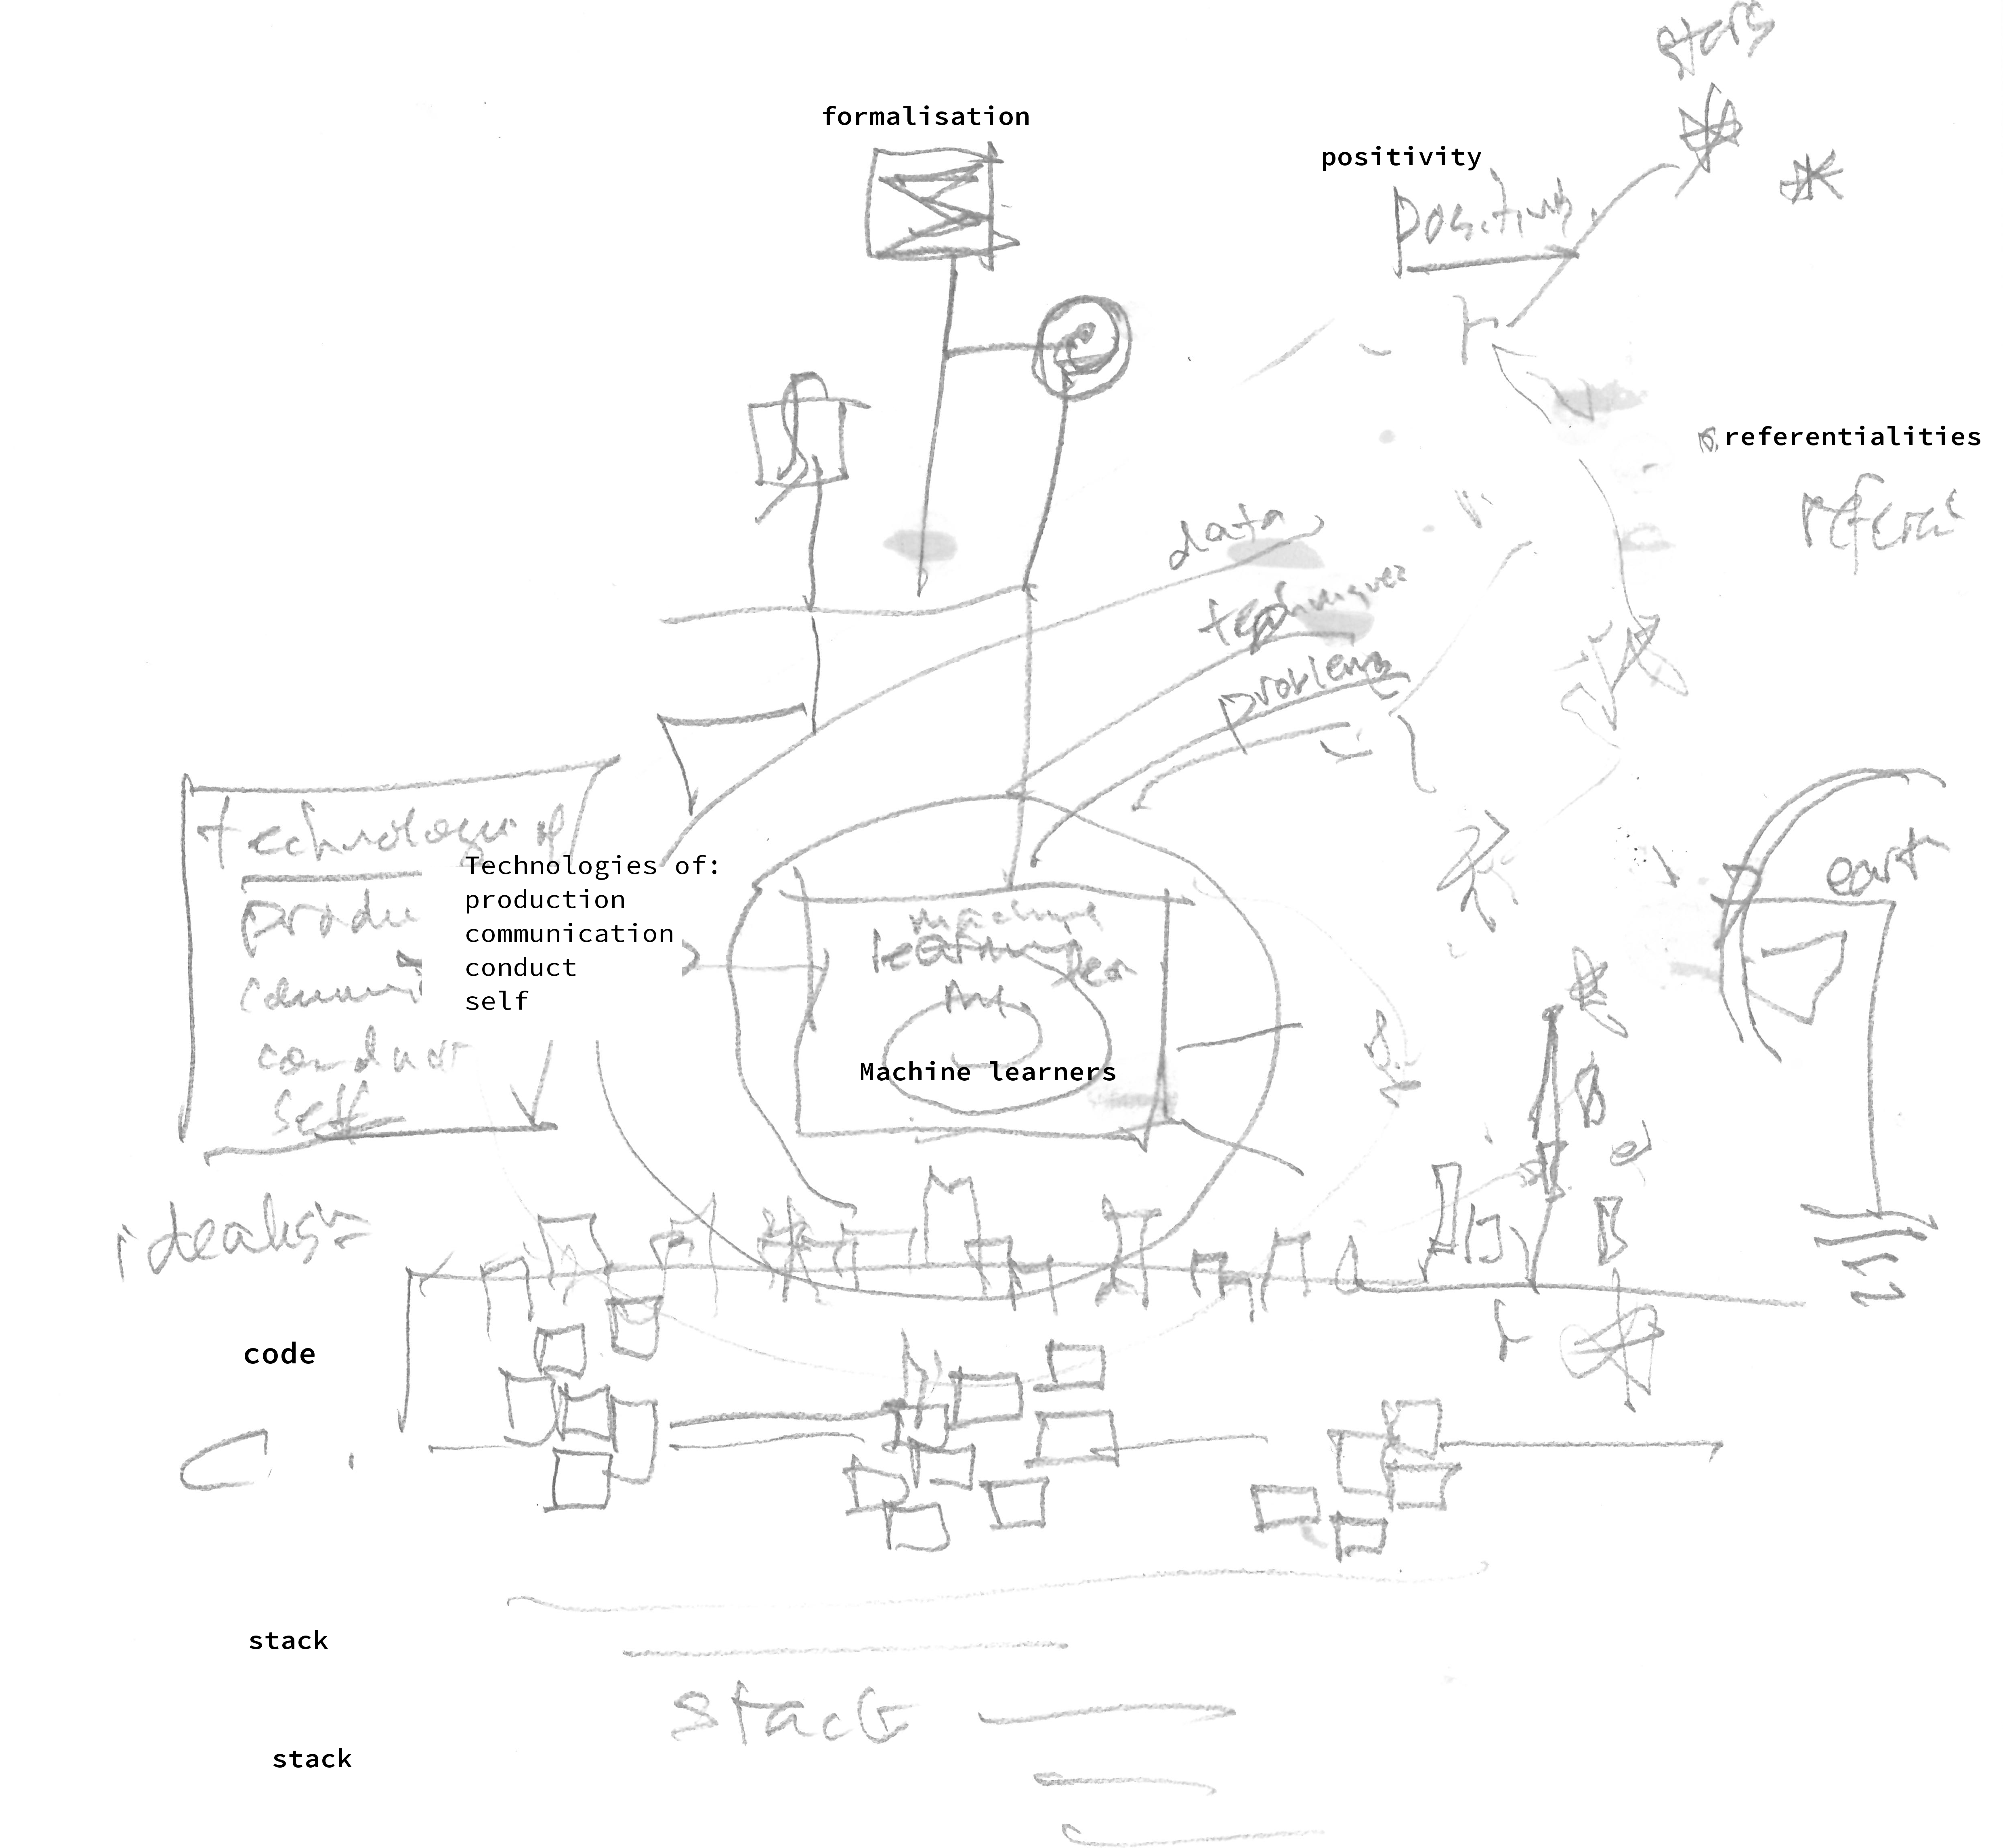
\includegraphics[width=0.9\textwidth]{figure/vast_diagram}
        \caption{Elements of learning to machine learn}
  \label{fig:vast_diagram}
\end{figure}

Some broadly shared topic structures help in any navigation of the
software libraries, pedagogical and research literatures. The textbooks,
the how-to recipe books
\autocites{Segaran_2007}{Kirk_2014}{Russell_2011}{Conway_2012} and the
online university courses on machine learning often have a similar topic
structure. \index{machine learning!topic structure of} They nearly
always begin with `linear models' (fitting a line to the data), then
move to logistic regression (a way of using the linear model to classify
binary outcomes; for example, spam/not-spam; malignant/benign;
cat/non-cat), and afterwards move to some selection of neural networks,
decision trees, support vector machine and clustering algorithms.
\index{linear regression} They add in some decision theory, techniques
of optimization, and ways of selecting predictive models (especially the
bias-variance trade-off).\footnote{They differ, however, in several
  important respects. Reading the \emph{Elements of Statistical
  Learning} textbook or one of machine learning books written for
  programmers (for example, \emph{Programming Collective Intelligence}
  or \emph{Machine Learning for Hackers}
  \autocites{Segaran_2007}{Conway_2012}) does not directly subject the
  reader to machine learning By contrast, doing a Coursera course on
  machine learning brings with it an ineluctable sense of being
  machine-learned, of oneself becoming an object of machine learning.
  The students on Coursera are the target of machine learning. Daphne
  Koller and Andrew Ng are leading researchers in the field of machine
  learning, but they also co-founded the online learning site
  \href{http://coursera.org}{Coursera}. \index{Coursera} As experts in
  machine learning, it is hard to imagine how they would not treat
  teaching as a learning problem. And indeed, Daphne Koller sees things
  this way:

  \begin{quote}
  There are some tremendous opportunities to be had from this kind of
  framework. The first is that it has the potential of giving us a
  completely unprecedented look into understanding human learning.
  Because the data that we can collect here is unique. You can collect
  every click, every homework submission, every forum post from tens of
  thousands of students. So you can turn the study of human learning
  from the hypothesis-driven mode to the data-driven mode, a
  transformation that, for example, has revolutionized biology. You can
  use these data to understand fundamental questions like, what are good
  learning strategies that are effective versus ones that are not? And
  in the context of particular courses, you can ask questions like, what
  are some of the misconceptions that are more common and how do we help
  students fix them? \autocite{Koller_2012} \index{Koller, Daphne}
  \end{quote}

  Whether the turn from `hypothesis-driven mode to the data-driven mode'
  has `revolutionized biology' is debatable (I return to this in a later
  chapter). And whether or not the data generated by my participation in
  Coursera's courses on machine learning generates data supports
  understanding of fundamental questions about learning also seems an
  open question. Nevertheless, the loopiness of this description
  interests and appeals to me. I learn about machine learning, a way for
  computer models to optimise their predictions on the basis of
  `experience'/data, but at the same time, my learning is learned by
  machine learners. This is not something that could happen very easily
  with a printed text, although versions of it happen all the time as
  teachers work with students on reading texts. While Coursera and other
  MOOCs promise something that mass education struggles to offer
  (individually profiled educational services), it also negatively
  highlights the possibility that machine learning in practice can,
  somewhat recursively, help us make sense of machine learning as it
  develops.} The topic structures have in recent years started to become
increasingly uniform. This coagulation around certain topics, problems
and mathematical formalisms is both something worth analyzing (since,
for instance, it definitely affects how machine learning is taken up in
different settings), but should not be taken as obvious or given since
it results from many iterations.

Amidst this avalanching machine learning materials and practice, a
single highly cited and compendious textbook, \emph{Elements of
Statistical Learning: Data Mining, Inference, and Prediction} dating
from from around 2000 and currently in its second edition
\autocite{Hastie_2009}, can be seen from almost any point of the
terrain.\footnote{The complete text of the book can be downloaded from
  the website \url{http://statweb.stanford.edu/~tibs/ElemStatLearn/}. At
  the end of short intensive course on data mining at the Centre of
  Postgraduate Statistics, Lancaster University, the course convenor,
  Brian Francis, recommended this book as the authoritative text. Some
  part of me rues that day. That book is a poisoned chalice; that is,
  something shiny, valuable but also somewhat toxic.}
\index{Elements of Statistical Learning@\textit{Elements of Statistical Learning}}
At least for archaeological purposes, I regard this book as an
assemblage, \index{archaeology!assemblages in} and a diagram that
presents many important statements, forms of visibility and relations
between forces at work in machine learning. The authors of the book,
Jeff Hastie, Rob Tibshirani and Jerome Friedman \index{Hastie, Jeff}
\index{Tibshirani, Rob} \index{Friedman, Jerome} are statisticians
working at Stanford and Columbia University.

\emph{Elements of Statistical Learning} is a massive textual object,
densely radiant with equations, tables, algorithms, graphs and
references to other scientific literature. From the first pages proper
of the book, almost every page has a figure or a table or a formal
algorithm (counting these together: 1670 equations; 291 figures; 34
tables; and 94 algorithms, giving a total of 2089 operational statements
threaded through the book). Equations rivet the text with mathematical
abstractions of varying sophistication. On each page of the book we are
seeing, reading, puzzling over and perhaps learning from the products of
code execution. The graphic figures are all produced by code. The tables
are mostly produced by code. The algorithms specify how to implement
code, and the equations diagram various operations, spaces and movements
that meant to run as code.

In the range of references, combinations of code, diagram, equation,
scientific disciplines and computational elements, and perhaps in the
somewhat viscous, inter-objectively diverse referentiality that impinges
on any reading of it, \emph{Elements of Statistical Learning} betrays
some hyperobject-like positivity \index{positivity}
\autocite{Morton_2013}. \index{hyperobject} It is an accumulation of
forms, techniques, practices, propositions and referential relations.
\emph{Elements of Statistical Learning} combines statistical science
with various algorithms to `learn from data' \autocite[1]{Hastie_2009}.
The data range across various kinds of problems (identifying spam email,
predicting risk of heart disease, recognising handwritten digits, etc.).
The learning takes the form of various machine learning techniques,
methods and algorithms (linear regression, k-nearest neighbours, neural
networks, support vector machines, the Google Page Rank algorithm,
etc.).

There are other juggernaut machine learning textbooks.
\index{machine learning!textbooks} Ethem Alpaydin's \emph{Introduction
to Machine Learning} \autocite{Alpaydin_2010} (a more computer
science-base account), Christopher Bishop's heavily mathematical
\emph{Pattern recognition and machine learning} \autocite{Bishop_2006},
Brian Ripley's luminously illustrated and almost coffee-table formatted
\emph{Pattern Recognition and Neural Networks} \autocite{Ripley_1996}
\index{Ripley, Brian}, Tom Mitchell's earlier artificial
intelligence-centred \emph{Machine learning} \autocite{Mitchell_1997}
\index{Mitchell, Tom}, Peter Flach's perspicuous \emph{Machine Learning:
The Art and Science of Algorithms that Make Sense of Data}
\autocite{Flach_2012} \index{Flach, Peter}, or further afield, the
sobering and laconic \emph{Statistical Learning for Biomedical Data}
\autocite{Malley_2011} all cover a similar range of data and approaches.
These and quite a few other recent machine learning textbooks display a
range of emphases, ranging from the highly theoretical to the very
practical, from an orientation to statistical inference to an emphasis
on computational processes, from science to commercial applications.

\section{Who reads machine learning
textbooks?}\label{who-reads-machine-learning-textbooks}

How does such textbook help us assess and engage with claim to learn
from data or to produce knowledge differently? While it certainly does
not comprehend everything taking place in and around machine learning,
it diagrams several \emph{elementary} tendencies or traits.
\index{\textit{Elements of Statistical Learning}!as diagram of abstraction}
It's readership as we will see is widespread. It has a heterogeneous
texture in terms of the examples, formalisms, disciplines and domains it
covers. It starkly renders the problems of making sense of mathematical
operations, diagrams and transformations carried on through calculation,
simulation, deduction or analysis. It draws on a matrix of operational
practices, particularly in the form of the \texttt{R} code it heavily
but somewhat latently relies on. In short, \emph{Elements of Statistical
Learning} presents a multi-faceted and somewhat monumental layering of
abstractive practice that might be open to archaeological inquiry.

\begin{verbatim}
## Error in sqliteSendQuery(con, statement, bind.data): error in statement: no such table: basic_refs
\end{verbatim}

\begin{verbatim}
## Error in eval(expr, envir, enclos): object 'res' not found
\end{verbatim}

\begin{verbatim}
## Error in stri_split_regex(string, pattern, n = n, simplify = simplify, : object 'sc' not found
\end{verbatim}

\begin{verbatim}
## Error in table(fields): object 'fields' not found
\end{verbatim}

\begin{verbatim}
## Error in rownames(tf): object 'tf' not found
\end{verbatim}

\begin{verbatim}
## Error in colnames(tf) = c("Citations", "Field"): object 'tf' not found
\end{verbatim}

\begin{verbatim}
## Error in xtable(tf, label = "tab:fields_citing_hastie", align = c("p{0.05\\textwidth}", : object 'tf' not found
\end{verbatim}

\begin{table}[ht]
\centering
\begingroup\tiny
\begin{tabular}{rrrrr}
  \hline
weight1 & weight2 & weight3 & error\_count & iteration \\ 
  \hline
0.00 & 0.00 & 0.00 &   0 &   1 \\ 
  0.10 & 0.00 & 0.00 &   1 &   1 \\ 
  0.20 & 0.00 & 0.10 &   2 &   1 \\ 
  0.30 & 0.10 & 0.10 &   3 &   1 \\ 
  0.30 & 0.10 & 0.10 &   0 &   2 \\ 
  0.40 & 0.10 & 0.10 &   1 &   2 \\ 
  0.50 & 0.10 & 0.20 &   2 &   2 \\ 
  0.50 & 0.10 & 0.20 &   2 &   2 \\ 
  0.40 & 0.00 & 0.10 &   0 &   3 \\ 
  0.50 & 0.00 & 0.10 &   1 &   3 \\ 
  0.50 & 0.00 & 0.10 &   1 &   3 \\ 
  0.60 & 0.10 & 0.10 &   2 &   3 \\ 
  0.50 & 0.00 & 0.00 &   0 &   4 \\ 
  0.60 & 0.00 & 0.00 &   1 &   4 \\ 
  0.60 & 0.00 & 0.00 &   1 &   4 \\ 
   \hline
\end{tabular}
\endgroup
\caption{Iterative change in weights as a perceptron learns the NAND function} 
\label{tab:nand_weights}
\end{table}

Who reads the \emph{Elements of Statistical Learning}?
\index{\textit{Elements of Statistical Learning}!readerships} It is
often cited by academic machine learning practitioners as an
authoritative guide. On the other hand, students participating in new
data science courses often come from different disciplinary backgrounds
and find the tome unhelpful (see the comment by students during an
introductory data science course documented in \autocite{Schutt_2013}).
Whether the citations are friendly or not, it is hard to find a field of
contemporary science, engineering, natural, applied, health and indeed
social science that has not cited it. A Thomson-Reuters Scientific `Web
of Science'(TM) search for references citing either the first or second
edition of \autocite{Hastie_2009} yields around 9000 results. These
publications sprawl across over 100 different fields of research.
\index{science!diversity of fields in machine learning} While computer
science, mathematics and statistics dominate, a very diverse set of
references comes from disciplines from archaeology, through fisheries
and forestry, genetics, robotics, telecommunications and toxicology
ripple out from this book since 2001. Table
\ref{tab:fields_citing_hastie} shows the top 20 fields by count. One
could learn something about the diagrammatic movement of machine
learners from that reference list, which itself spans biomedical,
engineering, telecommunications, ecology, operations research and many
other fields. While it is not surprising to see computer science,
mathematics and engineering appearing at highest concentration in the
literature, molecular biology, control and automation, operation
research, business and public health soon appear, suggesting something
of the propagating accumulation or positivity of machine learning.
\index{positivity!as form of accumulation}

\begin{figure}
  \centering
      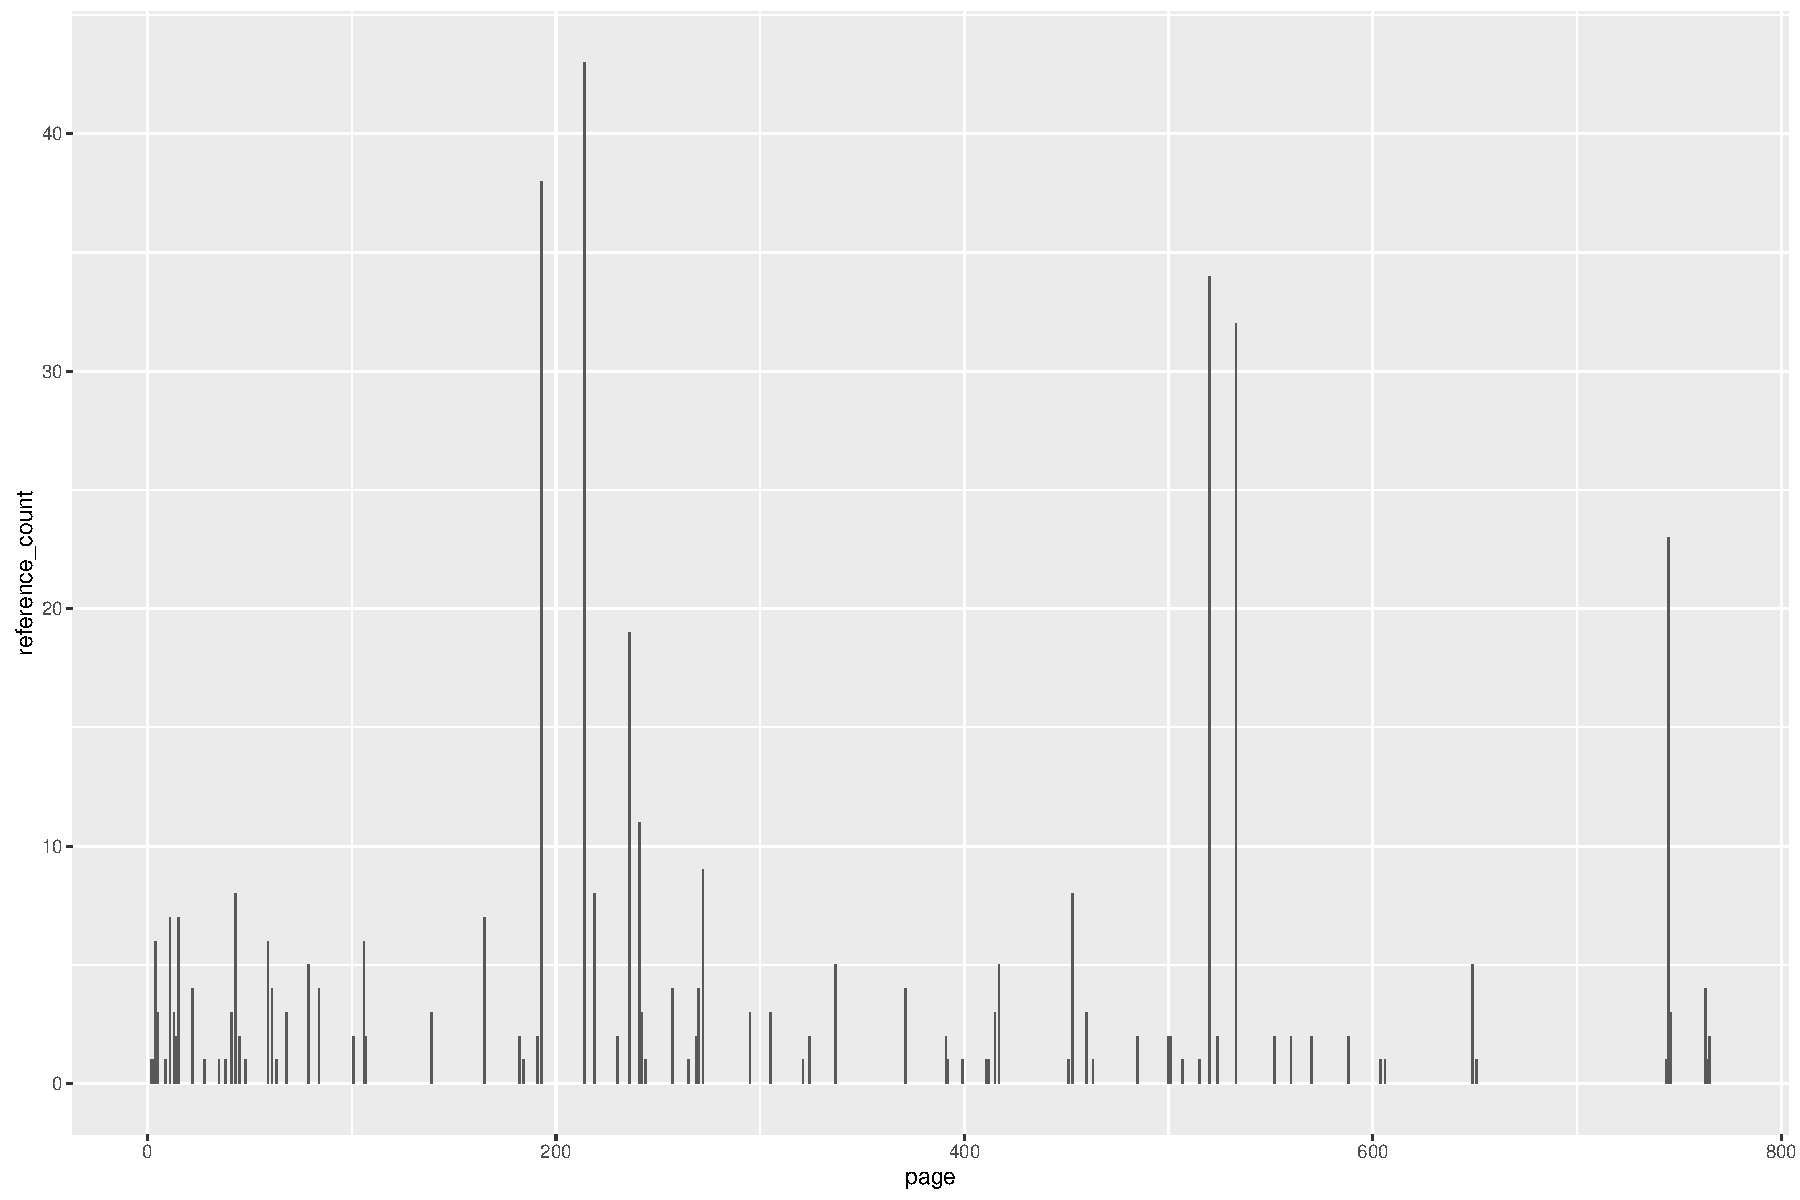
\includegraphics[width=0.9\textwidth]{figure/plot_hastie_pages-1.pdf}
        \caption[Pages cited from \textit{Elements of Statistical Learning }]{Pages cited from \textit{Elements of Statistical Learning }  by academic publications in all fields.}
  \label{fig:hastie_pages}
\end{figure}

So we know that \emph{Elements of Statistical Learning} passes into many
fields. But what do people read in the textual environment of book? In
general, the thousands of citations of the book themselves compose a
diagram of the book's intersection with different domains of knowledge.
The relative concentrations and sparsities of these citations suggest
there may be specific sites of engagement in the techniques, approaches
and machines that the book documents. Of the around 760 pages in the two
editions (\autocite{Hastie_2009} and \autocite{Hastie_2001}), around 83
distinct pages are referenced in the citing literature. As figure
\ref{fig:hastie_pages} indicates, certain portions of the book are much
more heavily cited than others. This distribution of page references in
the literature that cites \emph{Elements of Statistical Learning} is a
rough guide to how the book has been read in different settings. For
instance, the most commonly cited page in the book is page 553. That
page begins a section called `Non-negative Matrix Factorization',
\index{machine learner!Non-negative matrix factorization} a technique
frequently used to process digital images to compress their visual
complexity into a simpler set of visual signals
\autocite[553]{Hastie_2009}. (The underlying reference here is the
highly cited paper \autocite{Lee_1999}) Like \texttt{kittydar}, it, as
Hastie and co-authors write, `learns to represent faces with a set of
basis images resembling parts of faces' \autocite[555]{Hastie_2009}. (So
\texttt{kittydar}, which doesn't use NMF, might do better if it did,
because it could work just with parts of the images that lie somewhere
near the parts of a cat's face -- its nose, its eyes, its
ears.\index{machine learner!\texttt{kittydar}}) \index{face recognition}

Conversely, what do the authors of \emph{Elements of Statistical
Learning} read? The book gathers elements from many different quarters
and seeks to integrate them in terms of statistical theory. The
hyperobject-like aspect of the book comes from the thick weave of
equations, diagrams, tables, algorithms, bibliographic apparatus, and
numbers wreathed in typographic ornaments drawn from many other sources.
For instance, in terms of outgoing references or the literature that it
cites, \emph{Elements of Statistical Learning} webs together a field of
scientific and technical work with data and predictive models ranging
across half a century. The reference list beginning at page 699
\autocite[699]{Hastie_2009} runs for around 35 pages, and the five
hundred or so references there point in many directions. The weave of
these elements differs greatly from citational patterns in the
humanities or social sciences. Reading this book almost necessitates an
archaeological approach since it comprises so many parts and fragments.
\index{archaeology!reading practices in}

\begin{figure}
  \centering
      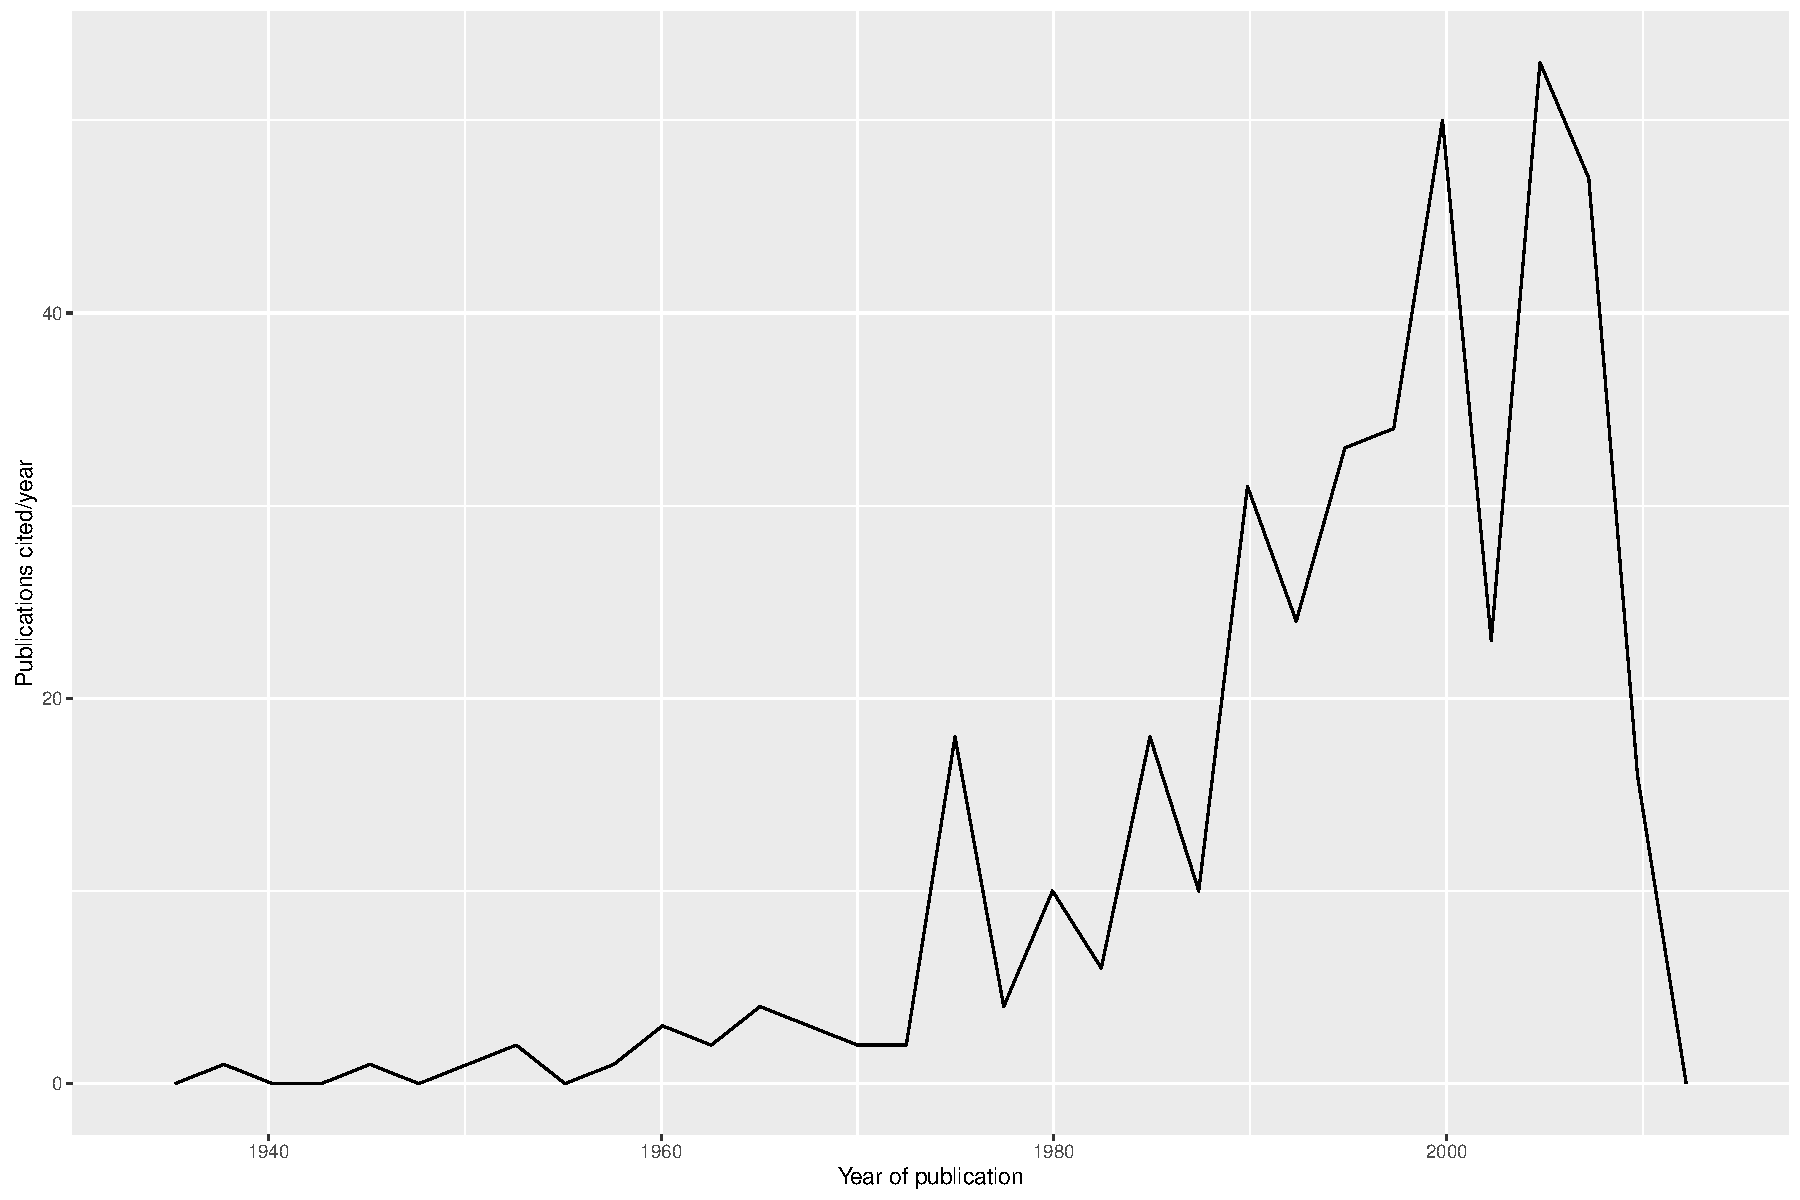
\includegraphics[width=0.9\textwidth]{figure/hastie_references-1.pdf}
        \caption[Publications cited in \textit{Elements of Statistical Learning}]{Publications cited in\textit{Elements of Statistical Learning}. The references range over almost 80 years, with peaks in late 1970s, late 1980s, mid-1990s and mid-2000s. These peaks relate to different mixtures of cybernetics, statistics, computer science, medicine, biology and other fields running through machine learning. Regression-related publications form the main body of citation. }
  \label{fig:hastie_cited_refs}
\end{figure}

The citational fabric of \emph{Elements of Statistical Learning} is
woven with different threads, some reaching back into early twentieth
statistics, some from post-WW2 cybernetics, many from information theory
and then in the 1980s onwards, increasingly, from cognitive science and
computer science (see figure \ref{fig:hastie_cited_refs} to get some
sense of their distribution over time). While some of these references
either point to Hastie, Tibshirani or Friedman's own publications, or
that of their statistical colleagues, the references rove quite widely
in other fields and over time. \emph{Elements of Statistical Learning}
as a text is processing, assimilating and recombining techniques,
diagrams and data from many different places and times. (The different
waves appearing in the references cited in \autocite{Hastie_2009} will
shape discussion in later chapters in certain ways; for instance, late
1990s biology is the topic of chapter \ref{ch:genome} and optimization
functions dating from the 1950s are discussed in chapter
\ref{ch:function}).

Both the inward and outward movements of citation suggest that
\emph{Elements of Statistical Learning}, like much in field of machine
learning, has a matrix-like character that constantly superimposes and
transposes elements across boundaries and barriers. The implication here
is that machine learning as a knowledge practice has a highly interwoven
texture, and in this respect differs somewhat from the classical
understandings of scientific disciplines as bounded by communities of
practice, norms and problems (as for instance, in Thomas Kuhn's account
of normal science \autocite{Kuhn_1996}. \index{Kuhn, Thomas} This
aggregate or superimposed character of machine learning should
definitely figure in any sense we make of it, and will inevitably affect
how critical thought might test itself against it.
\index{critical thought}.

\section{\texorpdfstring{\texttt{R}: a matrix of
transformations}{R: a matrix of transformations}}\label{r-a-matrix-of-transformations}

\index{programming languages!R|(} Although barely a single line of code
appears in \emph{Elements of Statistical Learning}, all of the learners
presented there are implemented in a single programming language,
\texttt{R}. Coding is the operational practice that links the different
planes and elements of machine learning in an operational formation.
\index{operational formation!code as operational practice in}
\index{code!as operational practice} The authors say `we used the R and
S-PLUS programming languages in our courses' \autocite[9]{Hastie_2009}
but many elements of the book derive from \texttt{R} code.\footnote{In a
  later book by some of the same authors with the very similar sounding
  title \emph{An Introduction to Statistical Machine Learning with
  Applications in \texttt{R}} \autocite{James_2013}, \texttt{R} does
  appear in abundance. This book, however, is much shorter and less
  inclusive in various ways. There are in any case many online manuals,
  guides and tutorials relating to \texttt{R} \autocite{Wikibooks_2013}.
  \index{programming languages!R!use of in machine learning textbooks}
  For present purposes, I draw mainly on semi-popular books such as
  \emph{R in a Nutshell} \autocite{Adler_2010}, \emph{The Art of
  \texttt{R} Programming} \autocite{Matloff_2011}, \emph{R Cookbook}
  \autocite{Teetor_2011}, \emph{Machine Learning with R}
  \autocite{Lantz_2013} or \emph{An Introduction to Statistical Learning
  with Applications in R} \autocite{James_2013}. These books are not
  written for academic audiences, although academics often write them
  and use them in their work. \index{machine learning!books!how-to} They
  are largely made up of illustrations and examples of how to do
  different things with different types of data, and their examples are
  typically oriented towards business or commercial settings, where,
  presumably, the bulk of the readers work, or aspire to work. Given a
  certain predisposition (that is, geekiness), these books and other
  learning materials can make for enjoyable reading. While they vary
  highly in quality, it is sometimes pleasing to see the economical way
  in which they solve common data problems. This genre of writing about
  programming specialises in posing a problem and solving it directly.
  In these settings, learning takes place largely through following or
  emulating what someone else has done with either a well known dataset
  (Fisher's \texttt{iris}) or a toy dataset generated for demonstration
  purposes. The many frictions, blockages and compromises that often
  affect data practice are largely occluded here in the interests of
  demonstrating the neat application of specific techniques. Yet are not
  those frictions, neat compromises and strains around data and machine
  learning precisely what we need to track diagrammatically? In order to
  demonstrate both the costs and benefits of approaching \texttt{R}
  through such materials, rather than through ethnographic observation
  of people using \texttt{R}, it will be necessary to stage encounters
  here with data that has not been completely transformed or cleaned in
  the interests of neatly demonstrating the power of a technique. One
  way to do this is by writing about code while coding.} The
proliferation of programming languages such as \texttt{FORTRAN} (dating
from the 1950s), \texttt{C} (1970s), \texttt{C++} (1980s), then
\texttt{Perl} (1990s), \texttt{Java} (1990s), \texttt{Python} (1990s)
and \texttt{R} (1990s), and computational scripting environments such as
Matlab, multiplied the paths along which machine learners move through
operational formations.\index{programming languages} It would be
difficult to comprehend the propagation of machine learners across
domains of science, business and government without paying attention to
coding practices. Even if textbooks and research articles are not read,
software packages and libraries for machine learning are used. Code has
a mobility that extends the diagrammatic practices of machine learning
into a variety of settings and places where the scientific reading
apparatuses of equations, statistical plots, and citations of research
articles would not be operative. \index{code!mobility of}

\begin{table}[!htb]
\centering
\begingroup\tiny
\begin{tabular}{rr}
  \hline
 & How often suggested \\ 
  \hline
testthat & 366 \\ 
  knitr & 167 \\ 
  knitr, rmarkdown & 103 \\ 
  MASS &  78 \\ 
  testthat, knitr, rmarkdown &  54 \\ 
  testthat, knitr &  48 \\ 
  RUnit &  38 \\ 
  knitr, rmarkdown, testthat &  35 \\ 
  knitr, testthat &  30 \\ 
  R.rsp &  30 \\ 
  lattice &  26 \\ 
  parallel &  26 \\ 
  ggplot2 &  18 \\ 
  mvtnorm &  16 \\ 
  survival &  14 \\ 
  rgl &  12 \\ 
  testthat, covr &  12 \\ 
  xtable &   9 \\ 
  akima &   8 \\ 
  dplyr &   7 \\ 
   \hline
\end{tabular}
\endgroup
\caption[ElemStatLearn suggest R packages]{R packages suggested by the ElemStatLearn package} 
\label{tab:elemstat_learn_suggests}
\end{table}

\textbackslash{}begin\{table\}{[}!htb{]} \centering
\begingroup\tiny
\begin{tabular}{rlr}
  \hline
 & Package & How often depended on \\ 
  \hline
methods & methods &  77 \\ 
  stats & stats &  33 \\ 
  survival & survival &  32 \\ 
  MASS & MASS &  27 \\ 
  mvtnorm & mvtnorm &  23 \\ 
  Matrix & Matrix &  13 \\ 
  ggplot2 & ggplot2 &  11 \\ 
  lattice & lattice &   9 \\ 
  rJava & rJava &   9 \\ 
  grid & grid &   7 \\ 
  igraph & igraph &   7 \\ 
  tcltk & tcltk &   7 \\ 
  XML & XML &   7 \\ 
  rgl & rgl &   6 \\ 
  graphics & graphics &   5 \\ 
  methods, stats & methods, stats &   5 \\ 
  nlme & nlme &   5 \\ 
  utils & utils &   5 \\ 
  vegan & vegan &   5 \\ 
  ape & ape &   4 \\ 
   \hline
\end{tabular}
\endgroup
\textbackslash{}caption{[}\texttt{ElemStatLearn} depends on R
packages{]}\{\texttt{R} packages depended on by the
\texttt{ElemStatLearn} package\} \label{tab:elemstat_learn_depends}
\textbackslash{}end\{table\}

How should we think of the \texttt{R} code in \emph{Elements of
Statistical Learning} in its operational specificity?
\index{programming languages!R!popularity of} Its growth is perhaps just
as important as its operation \autocite{Mackenzie_2014}. An open source
programming language, according to surveys of business and scientific
users, at the time of writing, \texttt{R} has replaced popular
statistical software packages such as SPSS, SAS and Stata as the
statistical and data analysis tool of choice for many people in
business, government, and sciences ranging from political science to
genomics, from quantitative finance to climatology
\autocite{RexerAnalytics_2015}. Developed in New Zealand in the
mid-1990s, and like many open source software projects, emulating
\texttt{S}, a commercialised predecessor developed at AT \& T Bell Labs
during the 1980s, \texttt{R} is now extremely widely used across life
and physical sciences, as well as quantitative social sciences. John
Chambers, the designer of \texttt{S}, was awarded the Association for
Computing Machinery (ACM) `Software System Award' in 1998 for `the S
system, which has forever altered how people analyze, visualize, and
manipulate data' \autocite{ACM_2013}. \index{Chambers, John} Many
undergraduate and graduate students today earn \texttt{R} as a basic
tool for statistics. Skills in \texttt{R} are often seen as essential
pre-requisite for scientific researchers, especially in the life
sciences. (In engineering, \texttt{Matlab} is widely used.) Research
articles and textbooks in statistics commonly both use \texttt{R} to
demonstrate methods and techniques, and create \texttt{R} packages to
distribute the techniques and sample data. Nearly all of these
publication-related software packages, including quite a few from the
authors of \emph{Elements of Statistical Learning} are soon or later
available from the `Comprehensive \texttt{R} Archive Network (CRAN)'
\autocite{CRAN_2010}. Estimates of its number of users range between
250000 and 2 million. Increasingly, \texttt{R} is integrated into
commercial services and products (for instance, SAS, a widely used
business data analysis system now has an \texttt{R} interface; Norman
Nie, one of the original developers of the SPSS package heavily used in
social sciences, now leads a business, Revolution, devoted to
commercialising \texttt{R}; \texttt{R} is heavily used at Google, at
FaceBook, and by quantitative traders in hedge funds; in 2013
\href{http://www.r-bloggers.com/r-usage-skyrocketing-rexer-poll/}{`R
usage is sky-rocketing'}; etc.). In general terms, \texttt{R} has a kind
of disciplinary polyglot currency as a form of expression, and exhibits
a fine-grained relationality with many different epistemic and
operational situations associated with machine learning.

Two early proponents of \texttt{R} and \texttt{S} describe the
motivation for the language:\index{programming languages!R and S}

\begin{quote}
The goal of the S language \ldots{} is ``to turn ideas into software,
quickly and faithfully'' \ldots{} it is the duty of the responsible data
analysts to engage in this process \ldots{} the exercise of drafting an
algorithm to the level of precision that programming requires can in
itself clarify ideas and promote rigorous intellectual scrutiny.
\ldots{} Turning ideas into software in this way need not be an
unpleasant duty. \autocite[2]{Venables_2002} \index{abstraction!in code}
\index{code!as abstraction}
\end{quote}

Bill Venables and Brian Ripley, statisticians working on developing
\texttt{S}, the almost identical commercial predecessor to \texttt{R},
wrote in the early 1990s of the responsibility of data analysts to write
not just use software. \index{Ripley, Brian} \index{Venables, Bill} They
write `software' here not in the sense of a product, but in the sense
that today would more likely be called `code.' Their sense of coding and
programming as clarifying and concretising ideas with precision -- as
abstractions -- has thoroughly taken hold in contemporary data analysis.
If code, as they suggest, entails a threshold of idealisation, it
differs from mathematical formalization in that it changes the positions
and relations of knowledge to include machines, devices and
infrastructures.

While the view that code is a precise expression of ideas makes sense,
it does not capture the relational complexity of \texttt{R} code as it
operates in a setting such as \emph{Elements of Statistical Learning}.
In machine learning, code, along with mathematics, is a primary
operational form that ideas take as they become machine learners. But
code as an expressive operation by which `an individual formulates an
idea' or as `a rational activity that may operate in a system of
inference' \autocite[117]{Foucault_1972} does not exhaust and should not
be conflated with operational practice in machine learning.
\index{operational practice} Similarly, the intersection of \texttt{R}
with machine learning also lies somewhat at odds with Pedro Domingos'
characterisation of machine learning as a shift away from people
building to learners growing programs.

\begin{lstlisting}[language=R, caption={Install packages in \texttt{R}}, label={lst:install_package}]
`install.packages('ElemStatLearn', dependencies='Suggests', repos = 'http://cran.us.r-project.org')
\end{lstlisting}

What in \texttt{R} (let alone other programming languages) overflows
both the ideas of code as expression of ideas and code as automation?
Alongside expression and automation, much \texttt{R} code furnishes a
matrix of practice crossing network infrastructures, display screens,
statistical techniques, software engineering architectures as well as
publication and documentation standards. For instance, the line of
\texttt{R} code shown in the listing \ref{lst:install_package} when
executed opens another way of reading \emph{Elements of Statistical
Learning} and getting a feel for the dragnet of practical relations and
infrastructural configurations running through it. Take the part of the
line
\texttt{dependencies\ =\ \textquotesingle{}Suggests\textquotesingle{}}.
When the line of code executes, the stipulation of \texttt{dependencies}
leads to a quite wide-ranging installation event that installs many
\texttt{R} packages. If the installation works (and that assumes quite a
lot of configuration work has already taken place; for instance,
installing a recent version of the \texttt{R} platform), then
\emph{Elements of Statistical Learning} is now augmented by various
pieces of code, and by various datasets that in some ways echo or mimic
the book but in other ways extend it operationally (see tables
\ref{tab:elemstat_learn_depends} and
\ref{tab:elemstat_learn_suggests}).\footnote{Most of the packages
  associated with the \texttt{ElemStatLearn}
  \index{R packages!\texttt{ElemStatLearn}} implement methods or
  techniques developed by Hastie, Tibshirani or Friedman, but some are
  much more generic. \texttt{MASS} for instance is highly cited
  \texttt{R} package. (Of the 9107 packages in the R CRAN system, 0
  depend on the library \texttt{MASS}, \index{R!packages!\texttt{MASS}}
  itself an adjunct to the influential and highly cited \emph{Modern
  Applied Statistics with S} \autocite{Venables_2002}, a textbook that
  presents many machine learning techniques using \texttt{S}
  \index{programming languages!S}, AT \& T Bell Labs commercial
  precursor to the open sourced \texttt{R}.
  \index{programming languages!R}) For our purposes, this hardly
  accidental mixing of academic or research work with a programming
  languages and its associated infrastructures is fortuitous. It allows
  us to transit between different strata of the social fields of
  science, engineering, health, medicine, business media and government
  more easily.}
\index{\textit{Elements of Statistical Learning}!code elements of} These
code elements are often stunningly specialised. As Karl Marx wrote of
the 500 different hammers made in Birmingham, `not only is each adapted
to one particular process, but several varieties often serve exclusively
for the different operations in one and the same process'
\autocite[375]{Marx_1986} \index{Marx, Karl!on hammers}. Something
similar holds in \texttt{R}: thousands of software packages in online
repositories suggest that a highly specialised division of labour and
possibly refined co-operative labour processes operate around data.
\index{R!packages!variety of}

Because of this almost incoherent plurality, and its labile status as
both a programming environment and a statistical analysis package,
\texttt{R} is an evocative object, to use the psychoanalyst Christopher
Bollas' term \autocite{Bollas_2008} \index{Bollas, Christopher}, an
object through which many different ways of thinking circulate. Standing
somewhere at the intersection of statistics and computing, modelling and
programming, many different disciplines, techniques, domains and actors
intersect in \texttt{R}. It engages immediately, practically and widely
with words, numbers, images, symbols, signals, sensors, forms,
instruments and above all abstract forms such as mathematical functions
like probability distributions and many different architectural forms
(vectors, matrices, arrays, etc.), as it employs data.
\index{programming languages!R|)} If, as Bollas suggests, `our
encounter, engagement with, and sometimes our employment of, actual
things is a \emph{way} of thinking' \autocite[92]{Bollas_2008},
\index{thinking} then it plausible that \texttt{R} not only gathers a
plurality of data practices -- working with measurements, numbers, text,
images, models and equations, with techniques for sampling and sorting,
with probability distributions and random numbers -- but that it
embodies the kernel of a mode of thought relevant to contemporary
realities. \index{critical thought!operational modes of}

\section{The obdurate mathematical glint of machine
learning}\label{the-obdurate-mathematical-glint-of-machine-learning}

If scientific research literature and operational \texttt{R} code
constitute the elements of an operational formation presented in
\emph{Elements of Statistical Learning}, what of the mathematics? While
references from many different places flow in and out of \emph{Elements
of Statistical Learning}, they are nearly all articulated in
mathematical form. Machine learning as a grouping of statements relies
heavily on mathematics. Given that mathematics is itself diverse and
multi-stranded, what kind of mathematics matters here? While later
chapters will explore some of the main mathematical practices (linear
algebra, statistical inference, etc.), machine learners in
\emph{Elements of Statistical Learning} coalesce around a single
exemplary technique: linear regression models or fitting a line to
points. \index{linear regression model|(} The linear regression model is
pivotal, not just in \emph{Elements of Statistical Learning} but in much
of the scientific and engineering literature. The linear regression
model pushes up some of the citational peaks in Figure
\ref{fig:hastie_cited_refs}. Even though it is an old technique dating
back to Francis Galton in the 1890s (see \autocite[chapter
8]{Stigler_1986}), \index{statistics!history of} it remains perhaps the
central working element of machine learning.
\index{machine learner!linear regression model}

\emph{Elements of Statistical Learning} acknowledges the statistical
legacy and inheritance in machine learning:

\begin{quote}
The linear model has been a mainstay of statistics for the past 30 years
and remains one of our most important tools. Given a vector of inputs
\(X^T = (X_1 , X_2, . . . , X_p)\), we predict the output \(Y\) via the
model \[\hat{Y} = \hat{\beta_0}  + \sum^p_(j=1)X_j\hat{\beta_j)}\] The
term \(\hat{\beta_0}\) is the intercept, also known as the \emph{bias}
in machine learning \autocite[11]{Hastie_2009}.
\end{quote}

In the course of the book, this mathematical expression appears in many
variations, iterations, expansions and modifications (`ridge
regression'; `least angle regression'; `project pursuit,' etc.). But
this introduction of the `mainstay of statistics,' the linear model,
already introduces a diagrammatic element -- the mathematical equation
-- that is perhaps the most prominent feature in the text.

Any reading of the book has to work out a way to traverse the forms show
in equation \ref{eq:linear_model}.

\begin{figure}
  \centering
      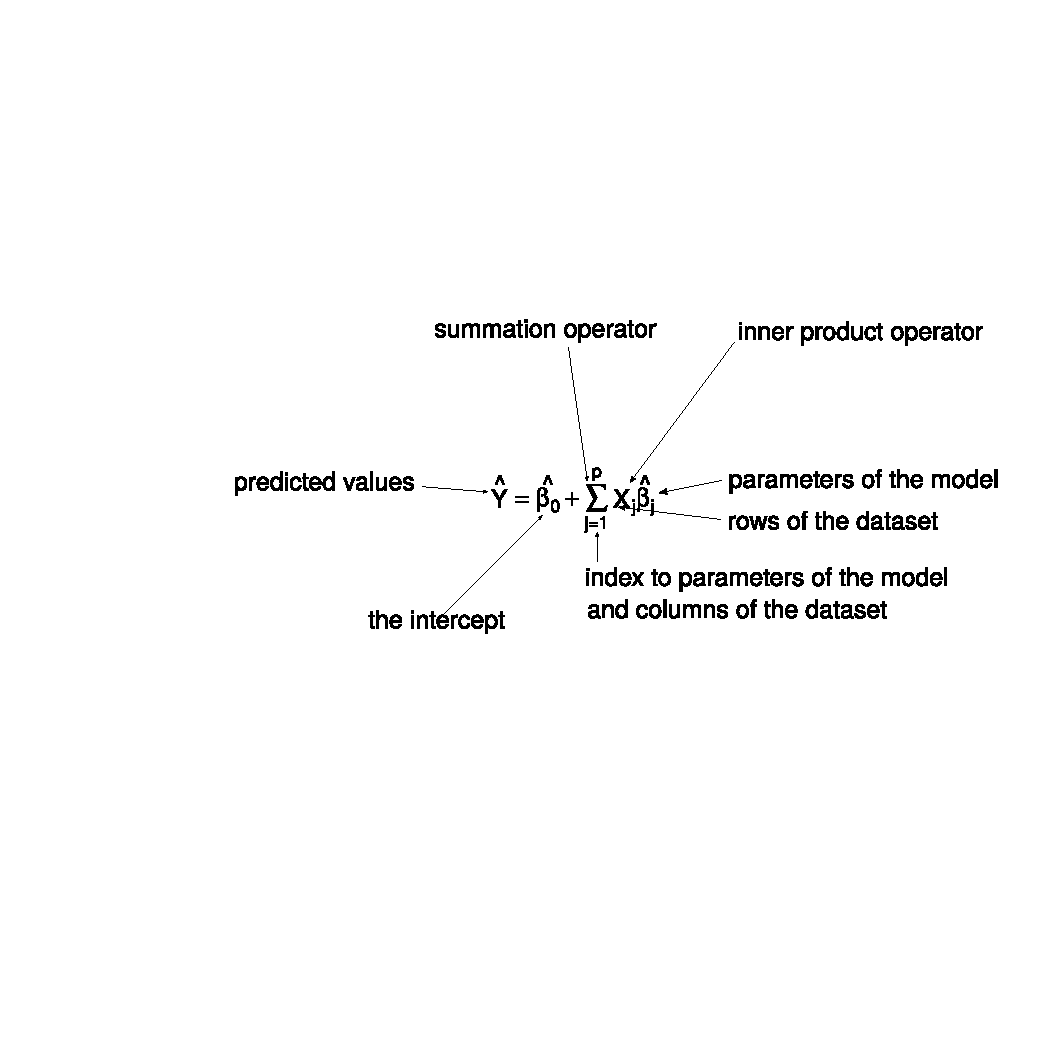
\includegraphics[width=0.9\textwidth]{figure/formula_labelled.pdf}
        \caption{The linear regression model}
  \label{fig:linear_model}
\end{figure}

In its relatively compressed typographic weave, expressions such as
Equation \ref{fig:linear_model} operationalize movements through data or
`a vector of inputs \(X^T\).' These expressions, which are not
comfortable reading for non-technical readers, are however worth looking
at carefully if we want to move `at the same level of abstraction as the
algorithm' \autocite{Pasquinelli_2015}.
\index{Pasquinelli, Paolo!on mathematics as abstraction} They can be
found in hundreds in \autocite{Hastie_2009}, but also in many other
places. While their presence distinguishes machine learning from parts
of computer science where mathematical equations are less common,
mathematical formalizations also allow the book to suture a panoply of
scientific publications and datasets in fields of statistics, artificial
intelligence and computer science. Along with the citations, the
graphical plots, and the code relationality, these equations are
integral connective tissue in machine learning.

In dealing with the obscuring dazzle of mathematical formalisation, I
find it useful here to follow Charles Sanders Peirce account of
mathematics. \index{mathematics!diagrammatic character of} `Mathematical
reasoning,' he writes, `is diagrammatic' \autocite[206]{Peirce_1998}.
\index{Peirce, Charles Sanders} \index{diagram|(} For Peirce, we should
see mathematics, whether it takes an algebraic or geometrical form,
whether it appears in symbols, letters, lines or curves as diagrams. For
Peirce, a diagram is a kind of `icon.' \index{diagram!icon} The icon is
a sign that resembles the object it refers to: it has a relation of
likeness. What likeness appears in equation \ref{fig:linear_model}?
Peirce says: `many diagrams resemble their objects not all in their
looks; it is only in respect to the relations of their parts that their
likeness consists' \autocite[13]{Peirce_1998}. As we have seen in the
perceptron code, machine learners can be expressed in statements in a
programming language like \texttt{Python} or \texttt{R.} In code,
however, the relations between parts cannot be observed in the same way
as they can in the algebraic form. The `very idea of the art,' as Peirce
puts it \autocite[228]{Peirce_1992}, of algebraic expressions is that
the formulae can be manipulated, or that component elements can be moved
without much effort through substitutions, transformations and
variations. The graphic form of the expression include the various
classical Greek operator symbols such as \gls{$\sum$} or \gls{$\prod$},
as well as the letters \(x, y, z\) and the indices (indexical signs)
such as \(j\) \index{diagram!indexical} that appear in subscript or
superscript, as well as the spatial arrangement of all these elements in
lines and sometimes arrays. A variety of relations run between these
different symbols and spatial arrangements. For instance, in all such
expressions, the relation between the left hand side of the `=' and the
right hand side is very important. By convention, the left hand side of
the expression is the value that is predicted or calculated (the
`response' variable) and the right hand side are the input variables or
`features' that contribute data to the model or algorithm.
\index{data!as variable in equations} This spatial arrangement
fundamentally affects the design of algorithms. In the case of equations
\ref{eq:linear_model}, the `\^{}' over \(\hat{Y}\) symbolises a
predicted value rather than a value that can be known completely through
deduction, derivation or calculation. This distinction between predicted
and actual values organizes a panoply of different practices and
imperatives (for instance, to investigate the disparities between the
predicted and actual values -- machine learning practitioners spend a
lot of time on that problem).

The broad point is that the whole formulae is a diagram, or an icon that
`\emph{exhibits}, by means of the algebraical signs (which are not
themselves icons), the relations of the quantities concerned'
\autocite[13]{Peirce_1998}. Because diagrams suppress so many details,
they allow one to focus on a selected range of relations between parts.
This affordance of diagrammatic mathematical forms is extremely
important in the operational formation of machine learning. Diagrams can
diagram other diagrams. Operations can themselves become the subject of
operations. The nesting of diagram is highly generative since it allows
what Peirce calls `transformations' \autocite[212]{Peirce_1998} or the
construction of `a new general
predicate'\autocite[303]{Peirce_1992}.\footnote{Félix Guattari makes
  direct use of Peirce's account of diagrams as icons of relation in his
  account of `abstract machines' \autocite{Guattari_1984}. He writes
  that `diagrammaticism brings into play more or less de-territorialized
  trans-semiotic forces, systems of signs, of code, of catalysts and so
  on, that make it possible in various specific ways to cut across
  stratifications of every kind' \autocite[145]{Guattari_1984}.
  \index{Guattari, Félix!diagram as abstract machine}
  \index{diagram!diagrammaticism of the} Here the `trans-semiotic
  forces' include mathematical formulae and operations (such as the
  banking system of Renaissance Venice, Pisa and Genoa). They are
  trans-semiotic because they are not tethered by the signifying
  processes that code experience or speaking positions according to
  given stratifications such as class, gender, nation and so forth.
  While Guattari (and Deleuze in turn in their co-written works
  \autocite{Guattari_1988}) is strongly critical of the way which
  signification territorializes (we might think of cats patrolling,
  marking and displaying in order to maintain their territories), he is
  much more affirmative of diagrammatic processes. He calls them
  `a-signifying' to highlight their difference from the signifying
  processes that order social strata. He suggests that diagrams become
  the foundation for `abstract machines' and the `simulation of physical
  machinic processes.' Writing in the 1960s, Guattari powerfully
  anticipates the abstract machines and their associated diagrams that
  have taken shape and physical form in the succeeding decades.
  \index{abstraction!as diagram}} \index{diagram!transformation of}

While I seek to relate to the equations as diagrams, and will present a
selection of them (nowhere near as many as found in \emph{Elements of
Statistical Learning}) in the following pages, I am not assuming their
operation is transparent or fully legible. Just as much as the analysis
of a photograph, a literary work or an ethnographic observation, their
diagrammatic composition calls for repeated consideration. Peirce
advises not to begin with examples that are too simple: `in simple
cases, the essential features are often so nearly obliterated that they
can only be discerned when one knows what to look for'
\autocite[206]{Peirce_1998}. He also suggests `it is of great importance
to return again and again to certain features'
\autocite[206]{Peirce_1998}. Looking at these diagrammatic expressions
repeatedly might allows us to map something of how transformations,
generalisations or intensification flow across disciplinary boundaries,
across social stratifications, and sometimes, generate potentially
different ways of thinking about collectives, inclusion and belonging.

\section{CS229, 2007: returning again and again to certain
features}\label{cs229-2007-returning-again-and-again-to-certain-features}

If we were to follow Peirce's injunction to `return again and again to
certain features,' how would we do that? \emph{Elements of Statistical
Learning} is a difficult book to read in isolation (although it does pay
re-reading). Even after several years, the diagrammatic density of its
`elements' or statements (equations, citations, tables, datasets, plots)
leaves me with a refractory feeling of `not quite understanding.' This
feeling is inevitable because the book condenses finished work from
several disciplines, and partly because it seeks to organize a great
diversity of materials \emph{epistemically.} Indeed, the book might seen
as evidence that machine learning has crossed an epistemic threshold
formulated in a statistical apparatus.
\index{machine learning!epistemic threshold of} (The statistical aspects
of machine learning are the main topic of chapter \ref{ch:probability}).

Does a computer science course offer a more easily followed route?
Andrew Ng's course `Machine Learning' CS229 at Stanford
(http://cs229.stanford.edu/) might provide a supplementary path into
machine learning \autocite{Ng_2008}.\footnote{A heavily shortened
  version of this course has been delivered under the title `Machine
  Learning' on
  \href{https://class.coursera.org/ml-003/class/index}{Coursera.org}, a
  MOOC (Massive Open Online Course) platform.}
\index{Ng, Andrew!CS229 lectures} The course description runs as
follows:

\begin{quote}
This course provides a broad introduction to machine learning and
statistical pattern recognition. Topics include supervised learning,
unsupervised learning, learning theory, reinforcement learning and
adaptive control. Recent applications of machine learning, such as to
robotic control, data mining, autonomous navigation, bioinformatics,
speech recognition, and text and web data processing are also discussed
\autocite{Ng_2008}
\end{quote}

CS229 is in many ways a typical computer science pedagogical exposition
of machine learning. Machine learning expositions usually begin with
simple datasets and the simplest possible statistical models and machine
learners (linear regression \index{linear regression}), and then, with a
greater or lesser degree of attention to issues of implementation, move
through a succession of increasingly sophisticated and specialised
techniques. This pattern is found in many of the how-to books, in the
online courses, and in the academic textbooks, including
\autocite{Hastie_2009}.

\begin{figure}
  \centering
      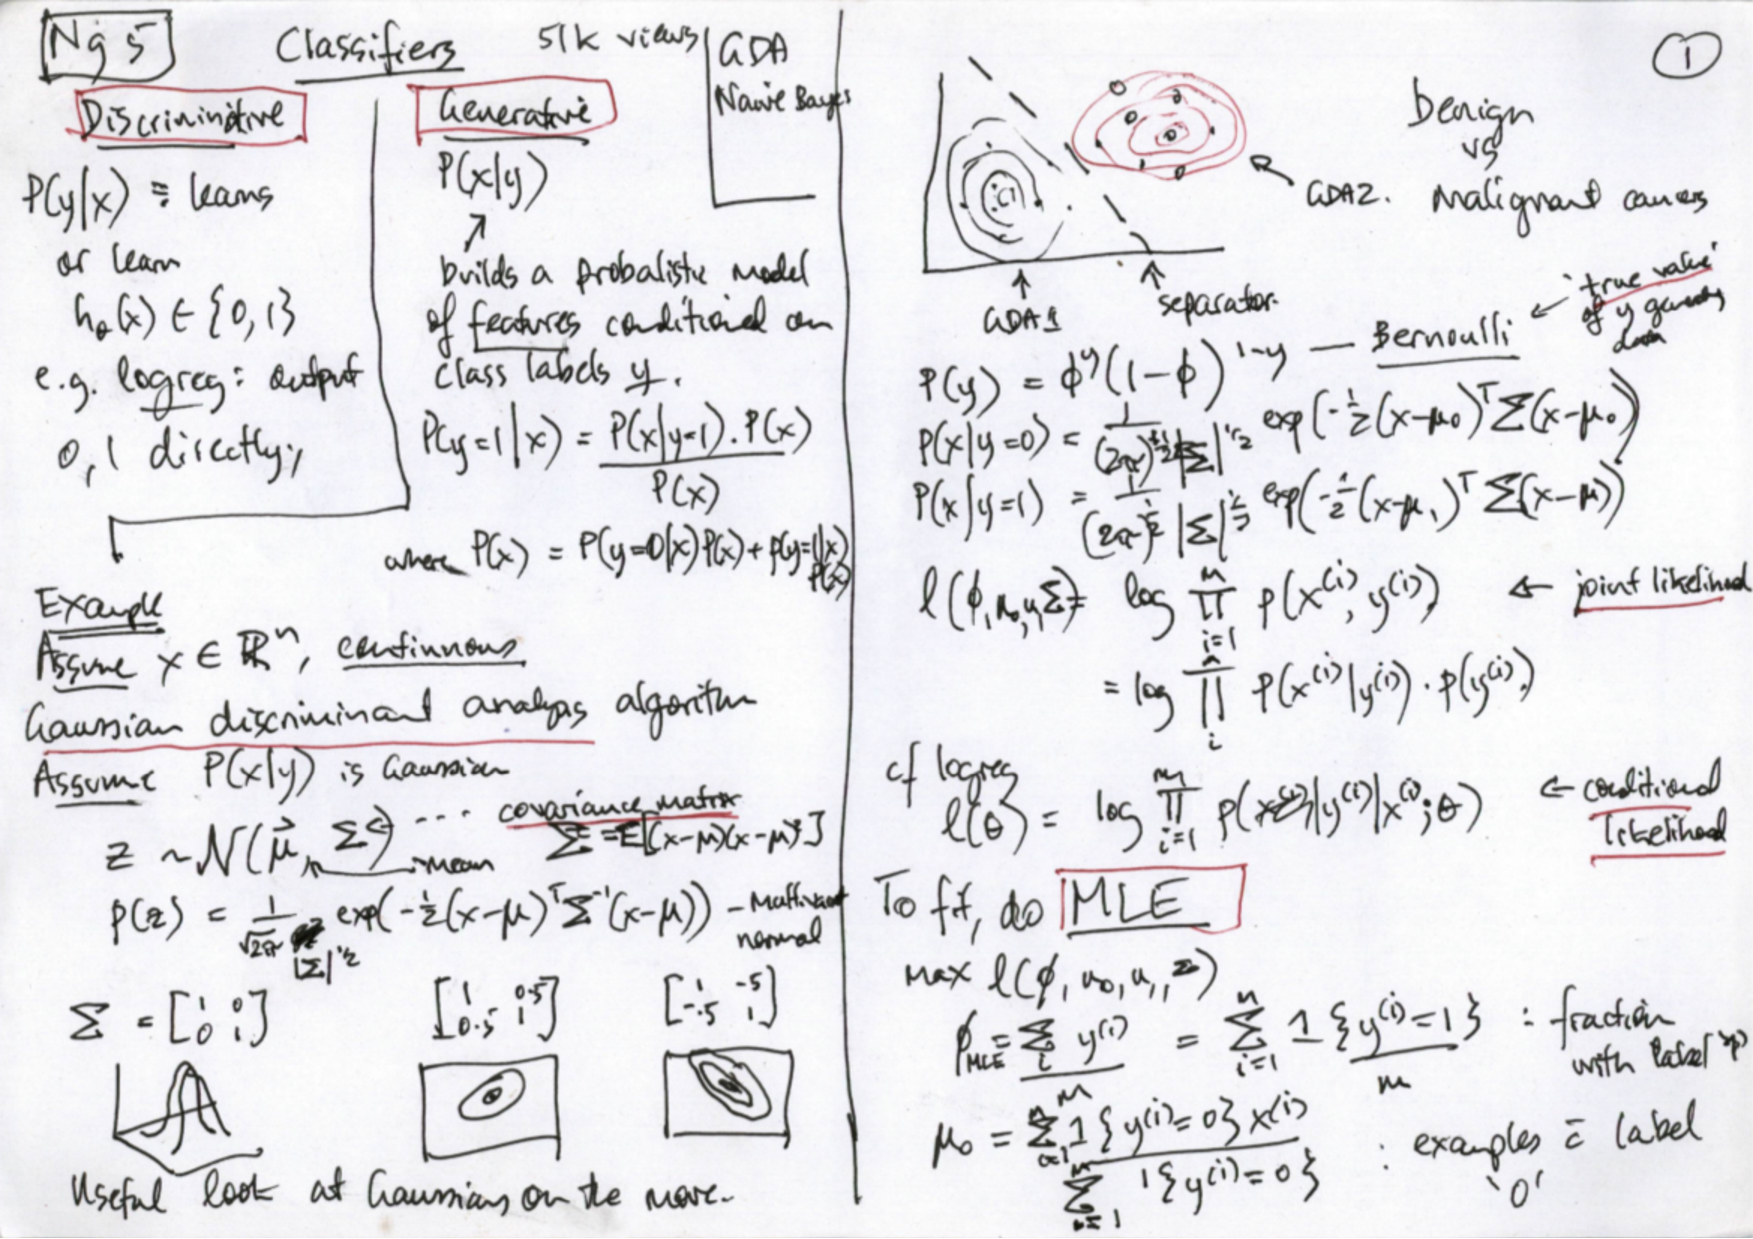
\includegraphics[width=0.9\textwidth]{figure/ng_lecture_5_generative_discriminative.pdf}
        \caption{Class notes lecture 5, Stanford CS229, 2007}
  \label{fig:class_notes}
\end{figure}

Ng's CS229 lectures differ from most other pedagogical materials in that
we see someone writing and deriving line after line of equations using
chalk on a blackboard. Occasionally, questions come from students in the
audience (not shown on the Youtube videos), but mostly Ng's
transcription of equations and other diagrams from the paper notes he
holds to blackboard continues uninterrupted.\footnote{After sitting
  through 20 hours of Ng's online lectures, and attempting some of the
  review questions and programming exercises, including implementing
  well-known algorithms using \texttt{R}, one comes to know datasets
  such as the San Francisco house price dataset and Fisher's
  \texttt{iris} \autocite{Fisher_1936} quite well. Like the textbook
  problems that the historian of science Thomas Kuhn long ago described
  as one of the anchor points in scientific cultures
  \autocite{Kuhn_1996}, these iconic datasets provide an entry point to
  the `disciplinary matrix' of machine learning. Through them, one gains
  some sense of how predictive models are constructed, and what kinds of
  algorithmic architectures and forms of data are preferred in machine
  learning.} Ng's Youtube anachronistic but popular lectures have a
certain diagrammatic density that comes from the many hours of chalked
writing he generates during the course deriving equations. In a time
when PowerPoint presentations or some other electronic textuality would
very much have been the norm (2007), why is a computer science
professor, teaching a fairly advanced postgraduate course, writing on a
chalkboard by hand?

Figure \ref{fig:class_notes} shows a brief portion of around 100 pages
of notes I made on this course. The act of writing down these equations
and copying the many hand-drawn graphs Ng produced was a deliberative
diagrammatic experiment in `returning again and again' to what is
perhaps overly hardened in \emph{Elements of Statistical Learning}. Like
the 50,000 or so other people who had watched this video, I partly
complied with Ng's injunction to `copy it, write it out, cover it, and
see if you can reproduce it' \autocite{Ng_2008d}. While it occasions
much writing and drawing, and many struggles to keep up with the
transformations and substitutions that Ng narrates as he writes, it
seems to me that writing out derivations, with all their substitutions
and variations, alongside the graphic sketches of intuitions about the
machine learners, accesses something of the \emph{diagrammatic
composition} of machine learning that is quite hard to track in
\emph{Elements of Statistical Learning}. \index{diagram!hand-drawn}
\index{mathematics!equations!derivation of} There the diagrammatic weave
between the expressions of linear algebra, calculus, statistics, and the
off-stage implementation in code is almost too tight to work with. In
Ng's CS229 lectures, by contrast, the weaving, while still complex, is
much more open. The lectures lack the citational tapestry of
\emph{Elements of Statistical Learning}. They are not able to wield the
datasets and the panoply of graphic forms found there, and virtually no
machine learning code appears on the blackboard (although the CS229
student assignments, also to be found online, are code implementations
of the algorithms and models). But Ng's lectures move more slowly, and
we begin to see some of the different groupings and associations
comprising the operational formation. More importantly perhaps, this
absorbing process of writing derivations might begin to transform ways
of thinking, saying and knowing. \index{diagram!hand-drawn}

\section{The visible learning of machine
learning}\label{the-visible-learning-of-machine-learning}

For a book with `learning' in its title, \emph{Elements of Statistical
Learning} has visibly little to say about how to learn machine learning.
\index{learning} `Learning' is briefly discussed on the first page of
\emph{Elements of Statistical Learning}, but the book hardly ever
returns to the topic or even that term explicitly. We learn on page 2
that a `learner' in machine learning is a model that predicts outcomes.
(As I discuss in chapter \ref{ch:function}, learning is comprehensively
understood in machine learning as finding a mathematical \emph{function}
that could have generated the data, and optimising the search for that
function as much as possible.) \index{learning!as function-finding} The
notion of learning in machine learning derives from the field of
artificial intelligence. The broad project of artificial intelligence,
at least as envisaged in its 1960s-1970s heyday as a form of symbolic
reasoning, is today largely regarded as a dead-end.
\index{artificial intelligence!relation to machine learning}

How then did learning get into the title of \emph{Elements of
Statistical Learning}? Does `learning' anthropomorphize statistical
modelling or computer programming? \index{learning} The so-called
`learning problem' and the theory of learning machines developed by
researchers in the 1960-1970s was largely based on work already done in
the 1950s on cybernetic devices such as the perceptron, the prototypical
neural network model developed by the psychologist Frank Rosenblatt in
the 1950s \autocite{Rosenblatt_1958}. \index{Rosenblatt, Frank}
\index{machine learner!perceptron|(} Drawing on the McCulloch-Pitts
model of the neurone and mathematical techniques of optimization
\autocite{Bellman_1961}, Rosenblatt implemented the perceptron, which
today would be called a single-layer neural network
\autocite[393]{Hastie_2009} as an electro-mechanical device at the
Cornell University Aeronautical Laboratory in 1957. For present
purposes, it is interesting to see what diagrams Rosenblatt used and how
they differ from contemporary diagrams.

\begin{figure}
  \centering
  \begin{subfigure}[b]{0.4\textwidth}
      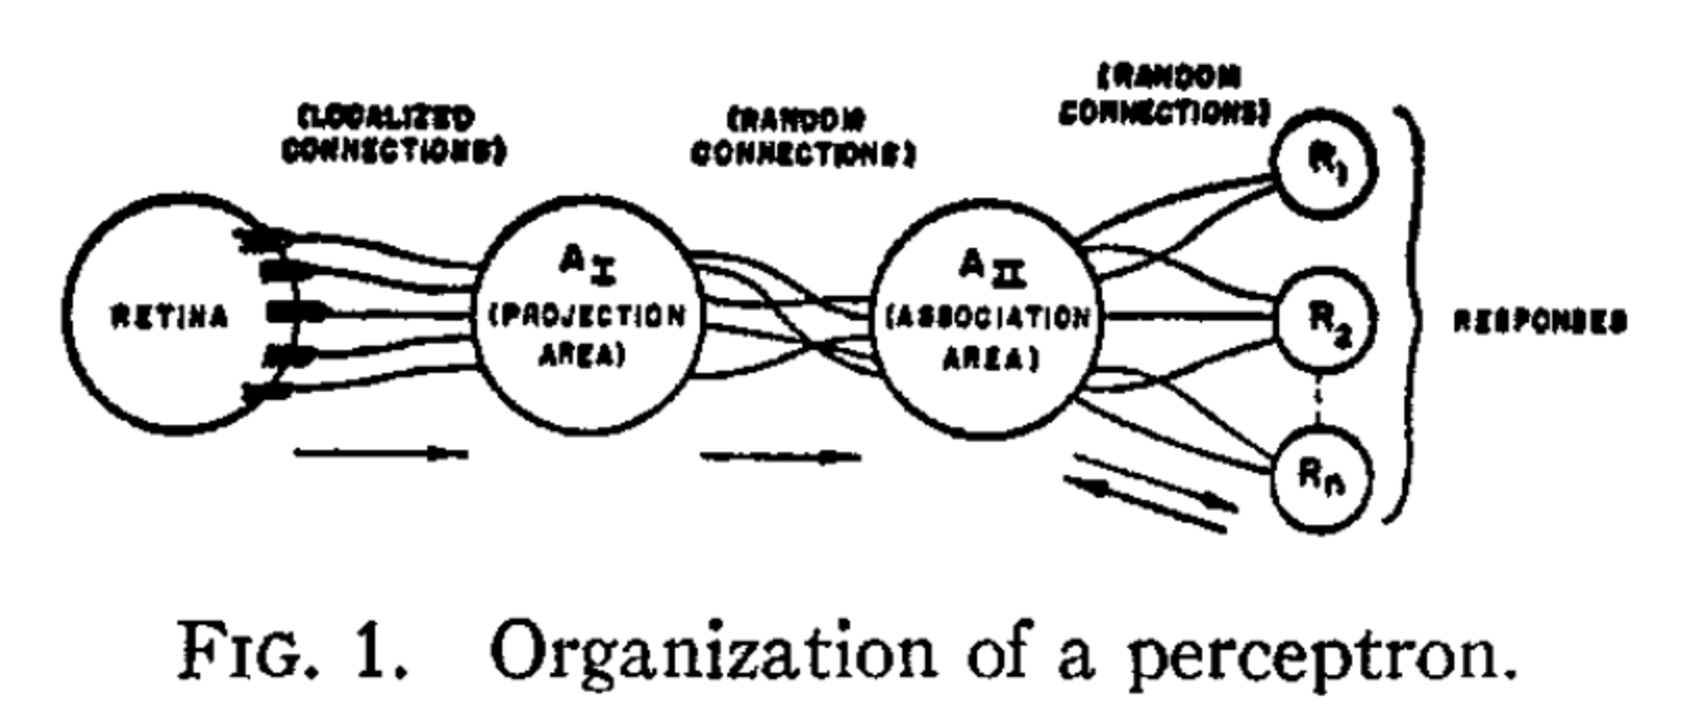
\includegraphics[width=\textwidth]{figure/perceptron_rosenblatt_1958_389.pdf}
        \caption{The neurological perceptron (Rosenblatt, 1958, 389)}
          \label{fig:perceptron_1958}
\end{subfigure}
  \begin{subfigure}[b]{0.3\textwidth}
      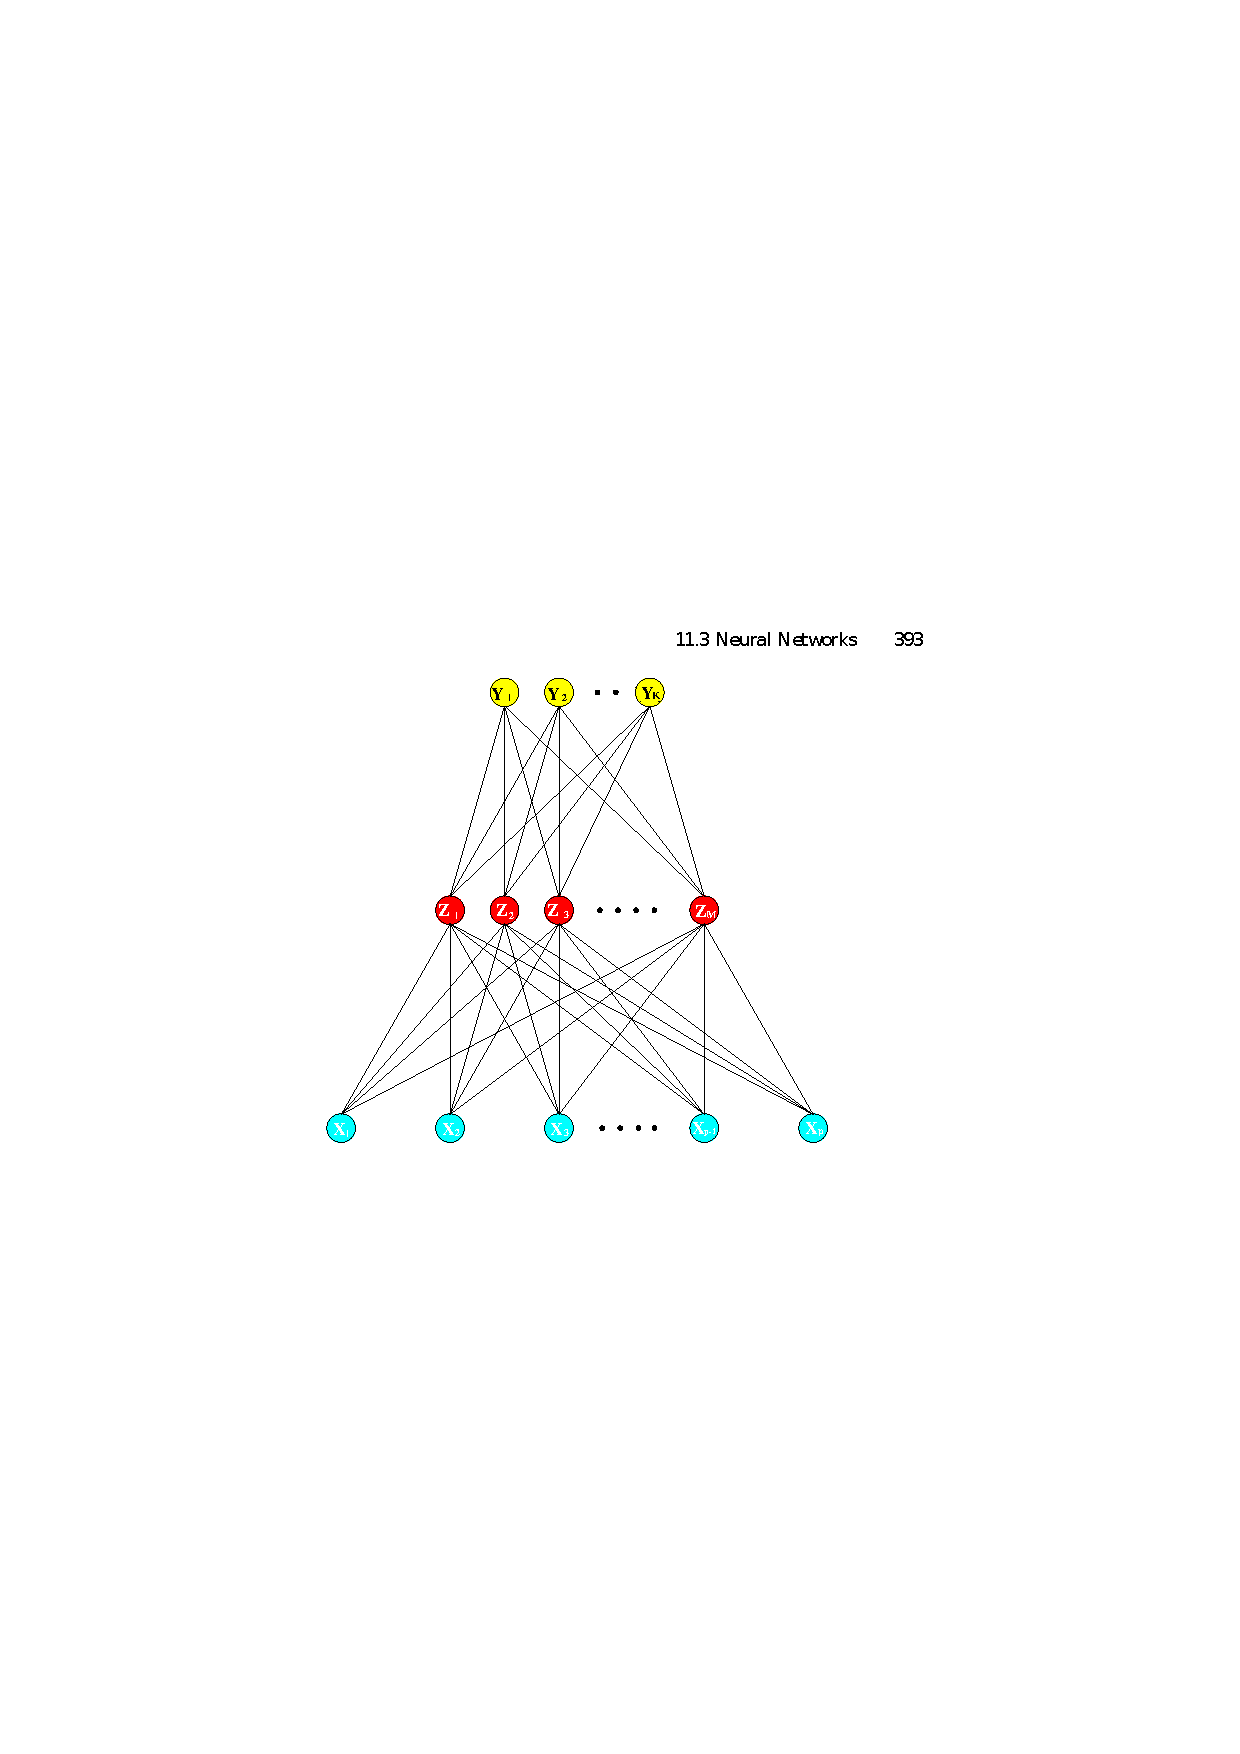
\includegraphics[width=\textwidth]{figure/hastie_ann_2009_393.pdf}
        \caption[Neural network from Hastie (2009)]{Neural network from Hastie (2009); Single layer feedforward artificial neural network.}
  \label{fig:hastie_ann}
    \end{subfigure}
    \label{figure:perceptron_ann}
    \caption{1958 perceptron and 2001 neural net compared}
\end{figure}

If we compare the diagram of Rosenblatt's perceptron shown in Figure
\ref{fig:perceptron_1958} to the typical contemporary diagram of a
neural network shown in Figure \ref{fig:hastie_ann}, the differences are
not that great in many ways. The diagram of a neural network found in
Rosenblatt's paper \autocite{Rosenblatt_1958} has no mathematical
symbols on it, but the one from \autocite{Hastie_2009} does.
Rosenblatt's retains neuro-cognitive-anatomical reference points
(retina, association area, projection area) whereas Hastie et. al.`s
replaces them with the symbols that we have already seen in play in the
expression for the linear model \ref{eq:linear_model}. What has happened
between the two diagrams? As Vladimir Vapnik, a leading machine learning
theorist, observes: 'the perceptron was constructed to solve pattern
recognition problems; in the simplest case this is the problem of
constructing a rule for separating data of two different categories
using given examples' \autocite[2]{Vapnik_1999}.
\index{Vapnik, Vladimir} While computer scientists in artificial
intelligence of the time, such as Marvin Minsky and Seymour Papert, were
sceptical about the capacity of the perceptron model to distinguish or
`learn' different patterns \autocite{Minsky_1969}, later work showed
that perceptrons could `learn universally'\footnote{In describing the
  entwined elements of machine learning techniques, and citing various
  machine learning textbooks, I'm not attempting to provide any detailed
  history of their development. My \gls{archaeology} \index{archaeology}
  of these developments does not explore the archives of institutions,
  laboratories or companies where these techniques took shape. It
  derives much more either from following citations back out of the
  highly distilled textbooks into the teeming collective labour of
  research on machine learning as published in hundreds of thousands of
  articles in science and engineering journals, or from looking at,
  experimenting with and implementing techniques in code. For instance,
  \autocite{Olazaran_1996} offers a history of the perceptron
  controversy from a science studies perspective.
  \index{machine learner!perceptron!history of} During the 1980s,
  artificial intelligence and associated approaches (expert systems,
  automated decision support, neural networks, etc.) were a matter of
  some debate in the sociology and anthropology of science. The work of
  Harry Collins would be one example of this \autocite{Collins_1990},
  Paul Edwards on artificial intelligence and Cold War
  \autocite{Edwards_1996}, Nathan Ensmenger on chess
  \autocite{Ensmenger_2012}, and Lucy Suchman on plans and expert
  systems \autocite{Suchman_1987} would be others. Philosophers such as
  Hubert Dreyfus (\emph{What Computers Can't Do}
  \autocites{Dreyfus_1972}{Dreyfus_1992} had already extensively
  criticised AI.
  \index{artificial intelligence!philosophical critiques of} In the
  1990s, the appearance of new forms of simulation, computational fields
  such as a-life and new forms of robotics such as Rodney Brook's much
  more insect-like robots at MIT attracted the interest of social
  scientists \autocite{Helmreich_2000} amongst many others. Sometimes
  this interest was critical of claims to expertise (Collins), and at
  other times, interested in how to make sense of the claims without
  foreclosing their potential novelty (Helmreich). By and large, I don't
  attend to controversies in machine learning as a scientific field, and
  I don't directly contest the epistemic authority of the proponents of
  the techniques. I share with Lucy Suchman an interest in how the
  `effect of machine-as-agent is generated' and in how `translations
  \ldots{} render former objects as emergent
  subjects'\autocite[2]{Suchman_2006}.
  \index{Suchman, Lucy!on machine-as-agent effect} I diverge around the
  site of empirical attention. I'm persevering with the diagrams in each
  of the following chapters in order to track the movement of tendencies
  that are not so visible in terms of either the controversies or the
  assumptions of agency embodied in many AI systems of the 1980s. The
  agency of machine learning, in short, might not reside so much in any
  putative predictive or classificatory power if manifests, but rather
  its capacity to mutate and migrate across contexts.
  \index{machine learning!agency of as mobility}}.\index{machine learner!perceptron|)}
For present purposes, the key point is not that neural networks have
turned out several decades later to be extremely powerful algorithms in
learning to distinguish patterns, and that intense research in neural
networks has led to their ongoing development and increasing
sophistication in many `real world' applications (see for instance, for
their use in sciences \autocite{Hinton_2006}, or in commercial
applications such as drug prediction \autocite{Dahl_2013} and above all
in the current surge of interest in `deep learning' by social media
platform and search engines such as Facebook and Google).
\index{machine learner!neural net} For our purposes, the important point
is that the notion of the learning machine began to establish an ongoing
diagonalization that transforms basic diagrammatic pattern through
substitutions of increasingly convoluted or nested operations. The whole
claim that machines `learn' rests on this diagrammatization that
recurrently and sometimes recursively transforms the icon of relations,
sometimes in the graphic forms shown above and more often in the
algebraic patterns.\index{diagrammatization}

The changes in graphics suggest transformations in the operational
formation. I am suggesting, then, that we should follow the
transformations associated with machine learning diagrammatically,
provided we maintain a rich understanding of diagram, and remain open to
multiple vectors of abstraction. \index{diagram|(} Following Peirce, we
might begin to see machine learning as a diagrammatic practice in which
different semiotic forms -- lines, numbers, symbols, operators, patches
of colour, words, images, marks such as dots, crosses, ticks and
arrowheads -- are constantly connected, substituted, embedded or created
from existing diagrams. The diagrams we have already seen from
\emph{Elements of Statistical Learning} - algebraic formulae and network
topology - don't exhaust the variations at all. Just a brief glance
through this book or almost any other in the field shows not only many
formulae, but tables, matrices, arrays, line graphs, contour plots,
scatter plots, dendrograms and trees, as well as algorithms expressed as
pseudo-code. The connections between these diagrams are not always very
tight or close. Learning to machine learning (whether you are a human
learner or a learner in the sense of a machine) means dancing between
diagrams. This dance is relatively silent and sometimes almost
motionless as signs slide between different diagrammatic articulations.
Diagrammatization offers then a way to track the ongoing project which
tries treat data like farmers treat crops (see epigraph from Domingos in
this chapter). To understand what machines can learn, we need to look at
how they have been drawn, designed, or formalised. But what in this work
of designing and formalising predictive models is like farming? Some
very divergent trajectories open up here. On the one hand, the diagrams
become machines when they are implemented. On the other hand, the
machines generate new diagrams when they function. We need to
countenance both forms of movement in order to understand any of the
preceding diagrams -- the algebraic expressions or the diagrams of
models such as the perceptron or its descendants, the neural network.
This means going downstream from the textbooks into actual
implementations and places where people, algorithms, and machines mingle
more than they do in the relatively neat formality of the textbooks.
Rather than history or controversies in the field, I focus on the
migratory patterns of methods, and the many configurational shifts
associated with their implementations as the same things appears in
different places. \index{diagram|)}

\section{The diagram of an operational
formation}\label{the-diagram-of-an-operational-formation}

Does machine learning radically change programming practice?
Programmability does change but only through gyrations between
epistemic, infrastructural and discursive heterogeneities practised and
practised in code. I have been suggesting that we can get a sense of the
heterogeneities and regularities of machine learning by treating
\emph{Elements of Statistical Learning} as a diagram
\index{\textit{Elements of Statistical Learning}!as diagram of operations}
that links and indexes the operations of machine learners in
publication, in computation, in code.
\index{hyperobject!machine learning as} Mapped through research
publications, pedagogical materials or code libraries in \texttt{R},
these operations form a primary field of expressions issuing from many
parts. These parts include the accumulation or positivity of scientific
literature with all its referentiality. \index{positivity} They include
mathematical derivation and formalization as an accelerated diagrammatic
movement. The parts include code as materially weaving of
infrastructures, conventions, standards, techniques, devices and
collective relations. \index{code!participation in machine learning}
Statements (especially linear algebra, calculus, statistics), problems
and techniques from multiple scientific disciplines (especially computer
science, but also biology, medicine and others), devices such as
computing platforms, data formats, and code repositories populate the
operational formation. The operational power of machine learning does
not stem from a single layer of abstraction. The diagrammatic forms of
movement we have begun to discern in the polymorphic \emph{Elements of
Statistical Learning} suggest key lines and paths worth following in
opening up that engagement. Like the perceptron calculating weights that
allow it to express the logic of the NAND function, we might first of
all turn to the table,\index{data!table} the ordering and aligning of
numbers on which nearly all machine learning depends.
